%TEMPLATE FILE
\documentclass{article}
\usepackage{graphicx} 
\usepackage{mathtools}
\usepackage{subcaption}
\usepackage[utf8x]{inputenc}
\usepackage{listings}
\usepackage{siunitx}
\usepackage{pdfpages}
\usepackage{pdflscape}
\usepackage{float}
\usepackage{xcolor}

\graphicspath{ {images/} }
\usepackage[obeyspaces]{url}
%\lstset{inputpath=C:/Users/Public/eclipse_workspace}
%\input{arduinoLanguage.tex}
\usepackage{color}   %May be necessary if you want to color links
\usepackage{hyperref}
\usepackage{titlesec}
\setcounter{secnumdepth}{4}

\hypersetup{
    colorlinks=true, % make the links colored
    linkcolor=blue, % color TOC links in blue
    urlcolor=red, % color URLs in red
    linktoc=all % 'all' will create links for everything in the TOC
    pdftitle={Sharelatex Example},
    bookmarks=true,
    pdfpagemode=FullScreen,
}
\hypersetup{
    colorlinks=true, % make the links colored
    linkcolor=blue, % color TOC links in blue
    urlcolor=blue, % color URLs in red
    linktoc=all % 'all' will create links for everything in the TOC
    pdftitle={Sharelatex Example},
    bookmarks=true,
    pdfpagemode=FullScreen,
    linkcolor=blue,
}

\definecolor{mGreen}{rgb}{0,0.6,0}
\definecolor{mGray}{rgb}{0.5,0.5,0.5}
\definecolor{mPurple}{rgb}{0.58,0,0.82}
\definecolor{backgroundColour}{rgb}{0.95,0.95,0.92}

\lstdefinestyle{CStyle}{
    %backgroundcolor=\color{backgroundColour},   
    commentstyle=\color{mGreen},
    keywordstyle=\color{magenta},
    numberstyle=\tiny\color{mGray},
    stringstyle=\color{mPurple},
    basicstyle=\footnotesize,
    breakatwhitespace=false,         
    breaklines=true,                 
    captionpos=b,                    
    keepspaces=true,                 
    numbers=left,                    
    numbersep=5pt,                  
    showspaces=false,                
    showstringspaces=false,
    showtabs=false,                  
    tabsize=2,
    language=C
}

\urlstyle{same}
\begin{document}
	\pagenumbering{gobble}
	\begin{titlepage}
		\centering
		\title{IOT Development platform \\ User manual \line(1,0){300}}
		\date{25.06.2019 \\ 
\includegraphics[width=0.1\linewidth]{HS_Weingarten} \\  }
		\author{\Large Hallmar Gauti Halldórsson\\ {Matrikel: 29404} \\ 
		\\ \Large Ravensburg Weingarten Universität } %author og fleirri upplysinga
	\end{titlepage}
	\maketitle
	\newpage
	\tableofcontents
	\newpage
	\pagenumbering{arabic}

\section{Abstract}
This the documentation for an Open-Source IOT development platform that is modular in nature. It is built to have one essential part and two parts that are flexible in nature. The essential part is the Power Supply board which uses a 3.7V LIPO battery to power the whole system through a vertical pin bus. 
The Power supply board can also charge the battery and has a Buck-Boost converter to get an additional 5V voltage line out of the 3.3V voltage line that is already regulated. 
\newline\newline
Then as of now there is the Microcontroller board which has a Feather Wi-Fi development platform from Adafruit and a 2 row 90° angled header that functions as a breakout for all of the pins of the Microcontroller as well as the 5V and 3.3V power supplies with some current limiting. 
\newline\newline
And finally there is the top most board which has an OLED that is controlled via I2C, three pushbuttons and a rotary encoder with a momentary switch. This is all connected to the Feather Microcontroller. 
\newline\newline
In the following document you will find the schematics, BOM's and important tips for assembling the platform. 
 %\ref{fig: pinout}.
 \section{Tips for assembling}
 
{\color{red} Take great care when soldering the small components labeled `U', they have to be oriented correctly. There is a small dot on the component which should line up with the dot on the silkscreen. If you cannot see it then use a magnifying glass}
\newline\newline
 There are a couple things to be aware of when assembling this platform, mainly because of the Vertical Bus system that it has.
It's simply some 2.54mm pitch header pins that connect the boards together, but soldering those pins correctly so that the boards fit together can be a bit tricky. 
The best way that I have found is to simply put all of the headers on the boards without soldering, screwing them all together(or atleast the first two boards) with the hex-standoffs, make sure that the headers are flush with their respected PCB and then solder the headers while the whole assembly is screwed together. Then you will get a perfectly vertical alignment of all the header pins. 
 \newpage
But before that you naturally have to solder the components, it is best to do it from the lowest component in size; Resistors, non-polarized capacitors, components labeled `U' then finally the USB connector and polarized capacitors. 
\newline\newline
To secure the battery I used some simple double sided tape. So far this has secured it pretty well. 
{\color{red} Be also aware that you need to solder two pads on the OLED screen before soldering it to the board because we are using it in I2C mode}, see the picture below. \\\\ If you want to use the frontpanel as is depicted in the section \hyperref[fig:HIDpic]{pictures for the HID Board.} then it's best to solder the header pins to the OLED, put the OLED in the PCB but DON'T SOLDER, then mount the frontpanel, put the device on it's front(frontpanel downwards), check if the OLED is straight and THEN you solder it to the PCB. The pins might be short so they might not go to the other side but just solder the pins on the other side of the PCB. You can see how I did it in the \hyperref[fig:HIDpic]{pictures for the HID Board.}
  \begin{figure}[H]
  	\centering
  	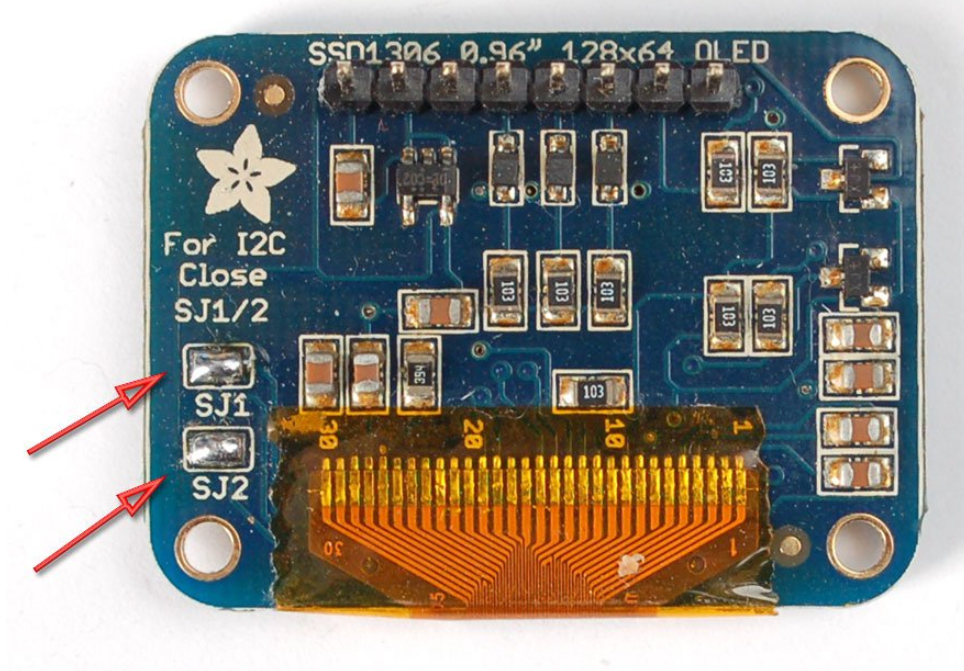
\includegraphics[width=1\linewidth]{oled.png}
  	\caption{I2C config for OLED}
 	 \label{fig:oled}
\end{figure}
%%%%%%%%%%%%%%%%%%%%
 \section{Vertical Bus}
 Here is a simple depiction of the vertical bus with the current versions of the Microcontroller board and HID board.
  \begin{figure}[H]
  	\centering
  	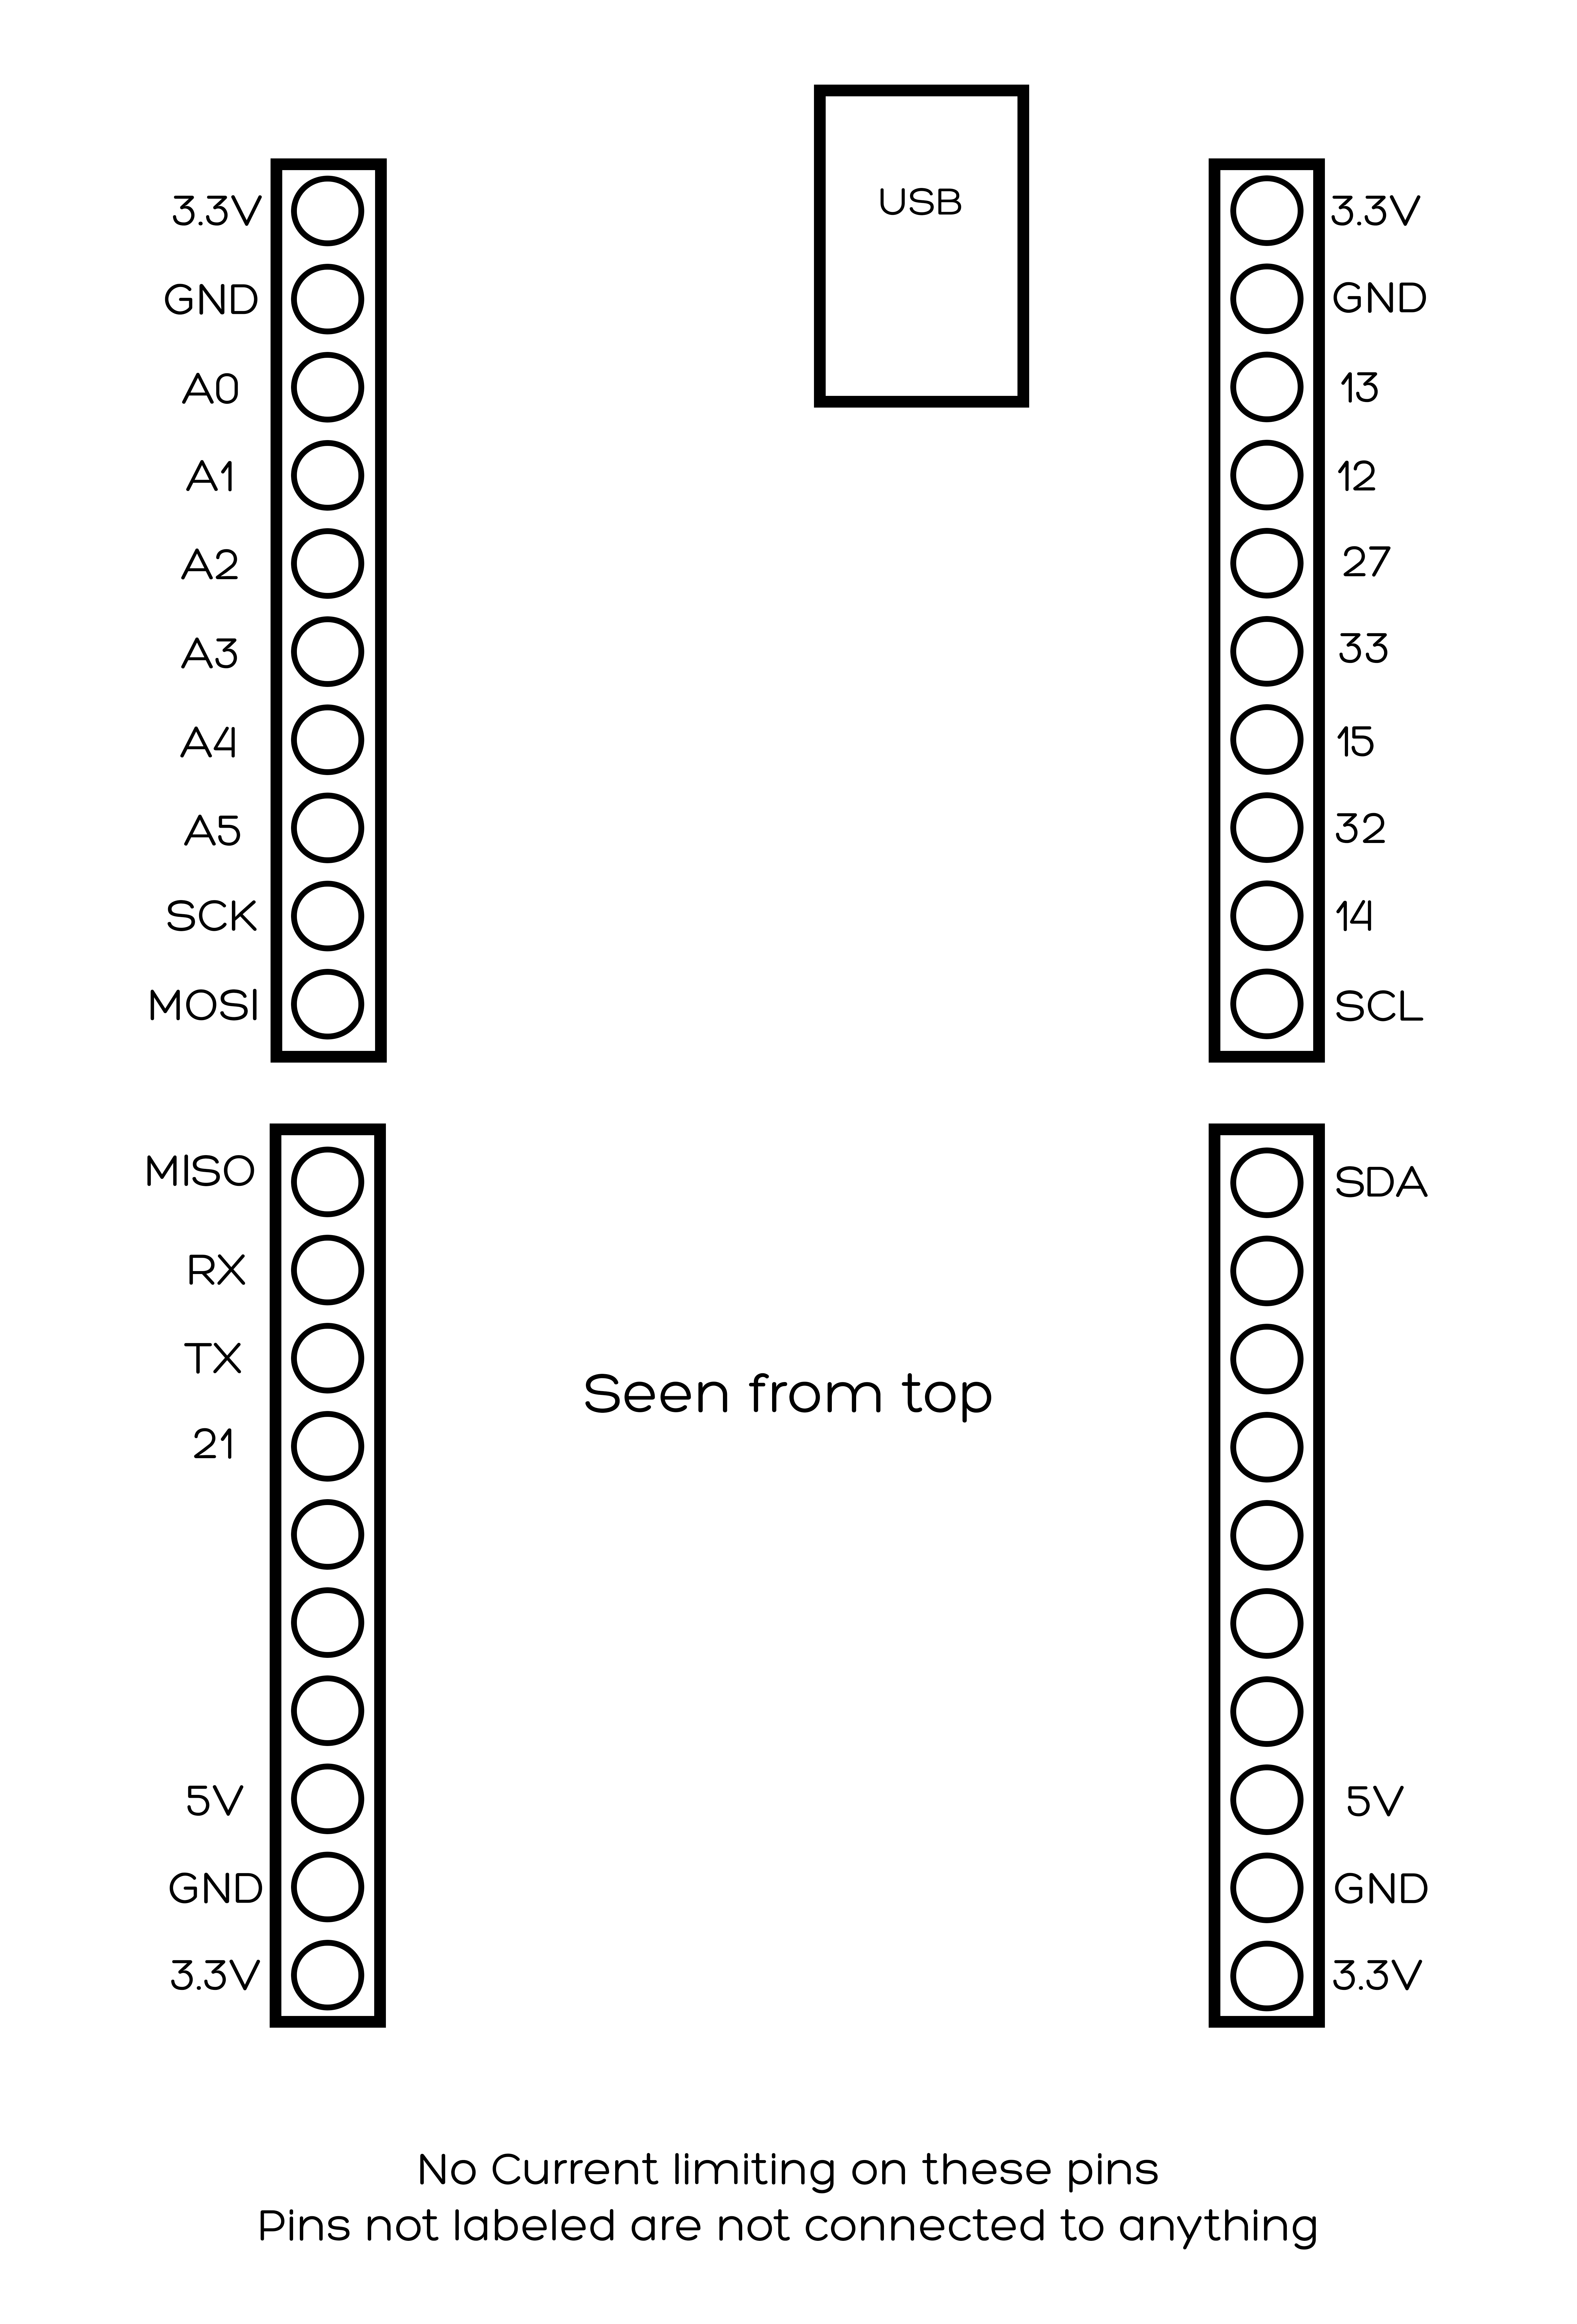
\includegraphics[width=0.7\linewidth]{vertical-bus-board.png}
  	\caption{Pinout for Vertical bus-board}
 	 \label{fig:vertical}
\end{figure}
\newpage
%%%%%%%%%%%%%%%%%%%%%
 \section{Battery/PSU PCB}
 This is the most important PCB since it powers the whole system and charges the battery. A Green LED indicates that power is ON and a red LED indicates that the battery is charging. The battery can charge while you use the system because there is a simple mosfet circuit that will disconnect the battery to the rest of the circuit except the battery charging part. \newline\newline
 The circuit also has a 3.3V to 5V buck-boost converter to be able to have 5V for prototyping purposes or for anything that requires 5V in the system. As of now everything runs on the 3.3V power supply. 
\newline
 Please take note that the Buck-Boost converter chip can only supply 100mA MAX. If you go above that or near it you might risk damage to the chip. 
 
 \subsection{BOM}
  \begin{center}
    \begin{tabular}{ |m{2em}|m{7em}|m{7em}|m{7em}|}
    \hline
	 \multicolumn{4}{|c|}{\textbf{Power Supply}} \\
	 \hline
       \textbf{Part} & \textbf{Value} & \textbf{Type} & \textbf{Package} \\ \hline
	C1 & 10$\mu$  & Electrolytic Capacitor & 0810 \\ \hline
	C2 & 10$\mu$  & Electrolytic Capacitor & 0810 \\ \hline
	C3 & 10$\mu$  & Electrolytic Capacitor & 0810 \\ \hline
	C4 & 100n & Capacitor & 1206 \\ \hline
	C5 & 10$\mu$  & Electrolytic Capacitor & 0810 \\ \hline
	C6 & 100n & Capacitor & 1206 \\ \hline
	C7 & 10$\mu$ & Electrolytic Capacitor & 0810 \\ \hline
	C8 & 10$\mu$ & Electrolytic Capacitor & 0810 \\ \hline
	
	D1 & MBRS130LT3 & Schottky Diode & SMB \\ \hline
	L1 & 10$\mu$ & Inductor & L3216C \\ \hline
	LED1 & RED  & LED & 3mm \\ \hline
	LED2 & GREEN & LED & 3mm \\ \hline
	Q1 & FDN360P & Transistor & SSOT-3\\ \hline
	
	R1 & 1k & Resistor & 1206 \\ \hline
	R2 & 100k & Resistor & 1206 \\ \hline
	R3 & 1k & Resistor & 1206 \\ \hline
	R4 & 100k & Resistor & 1206 \\ \hline
	R5 & 1k & Resistor & 1206 \\ \hline
	R6 & 220k & Resistor & 1206 \\ \hline
	R7 & 1M & Resistor & 1206 \\ \hline
	R8 & 100k & Resistor & 1206 \\ \hline
	R9 & 309k & Resistor & 1206 \\ \hline
	
	S1 & EG1213 & E-Switch & EG1213 \\ \hline
	U1 & AP2112K-3.3TRG1 & CMOS LDO & SOT-25-5 \\ \hline
	U2 & MCP73831 & LIPO Charger & SOT-23 \\ \hline
	U3 & MAX1834 & Buck-Boost Converter & SOT-23-6 \\ \hline
	X1 & PN61729-S & USB-B connector & PN61729-S \\ \hline
	SV1 & 10 pin & Female header & 2.54mm Pitch \\ \hline
	SV2 & 10 pin & Female header & 2.54mm Pitch \\ \hline
	SV3 & 10 pin & Female header & 2.54mm Pitch \\ \hline
	SV4 & 10 pin & Female header & 2.54mm Pitch \\ \hline
	CN1 & JST-2pin & 2 Pin connector & Adafruit \\ \hline
	
	Bat & 1200mA 3.7V & LIPO battery & Adafruit(see links section) \\ \hline
    \end{tabular}
     \end{center}
     \subsection{Placement}
         \begin{figure}[H]
  	\centering
  	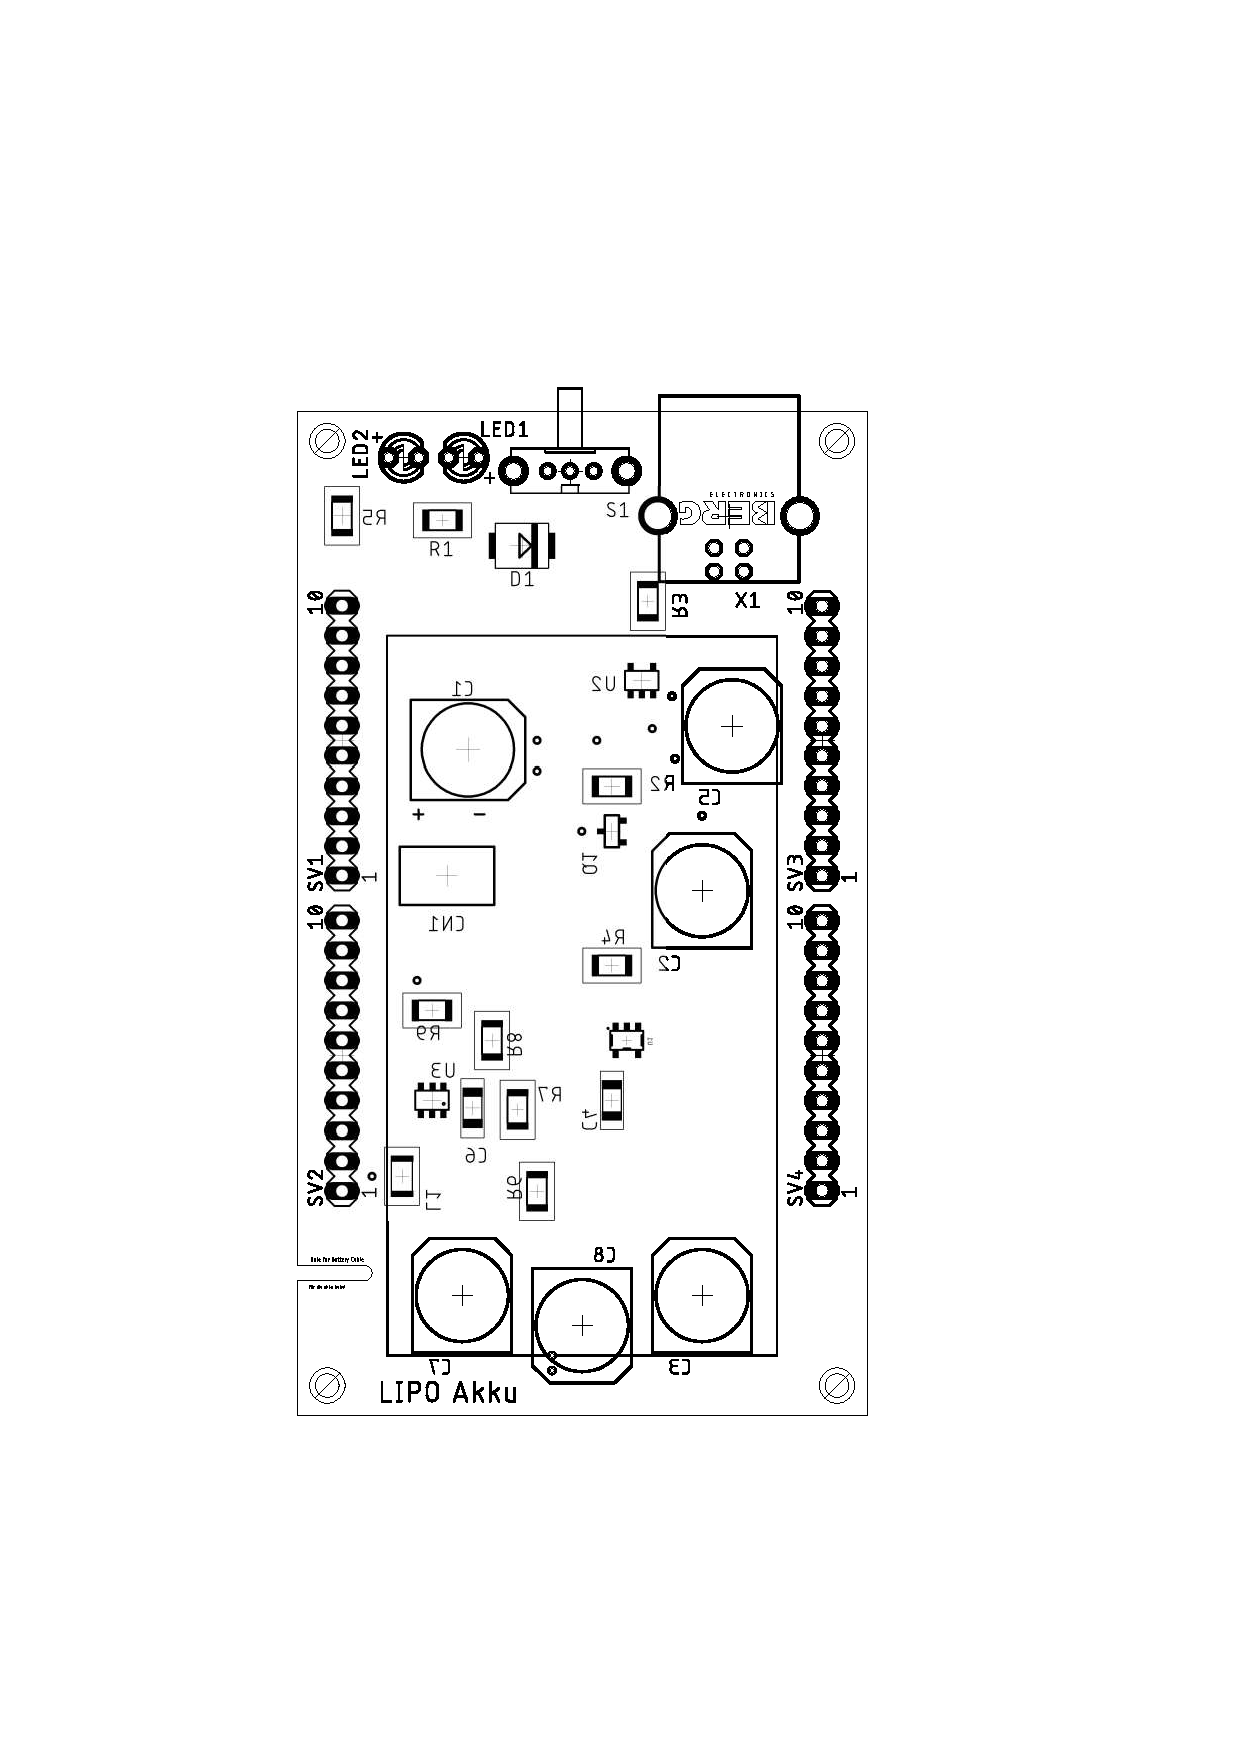
\includegraphics[width=1\linewidth]{battery-placement.pdf}
  	\caption{Placement for PSU board}
 	 \label{fig:place2}
\end{figure}

  \subsection{Schematic}
     \begin{figure}[H]
  	\centering
  	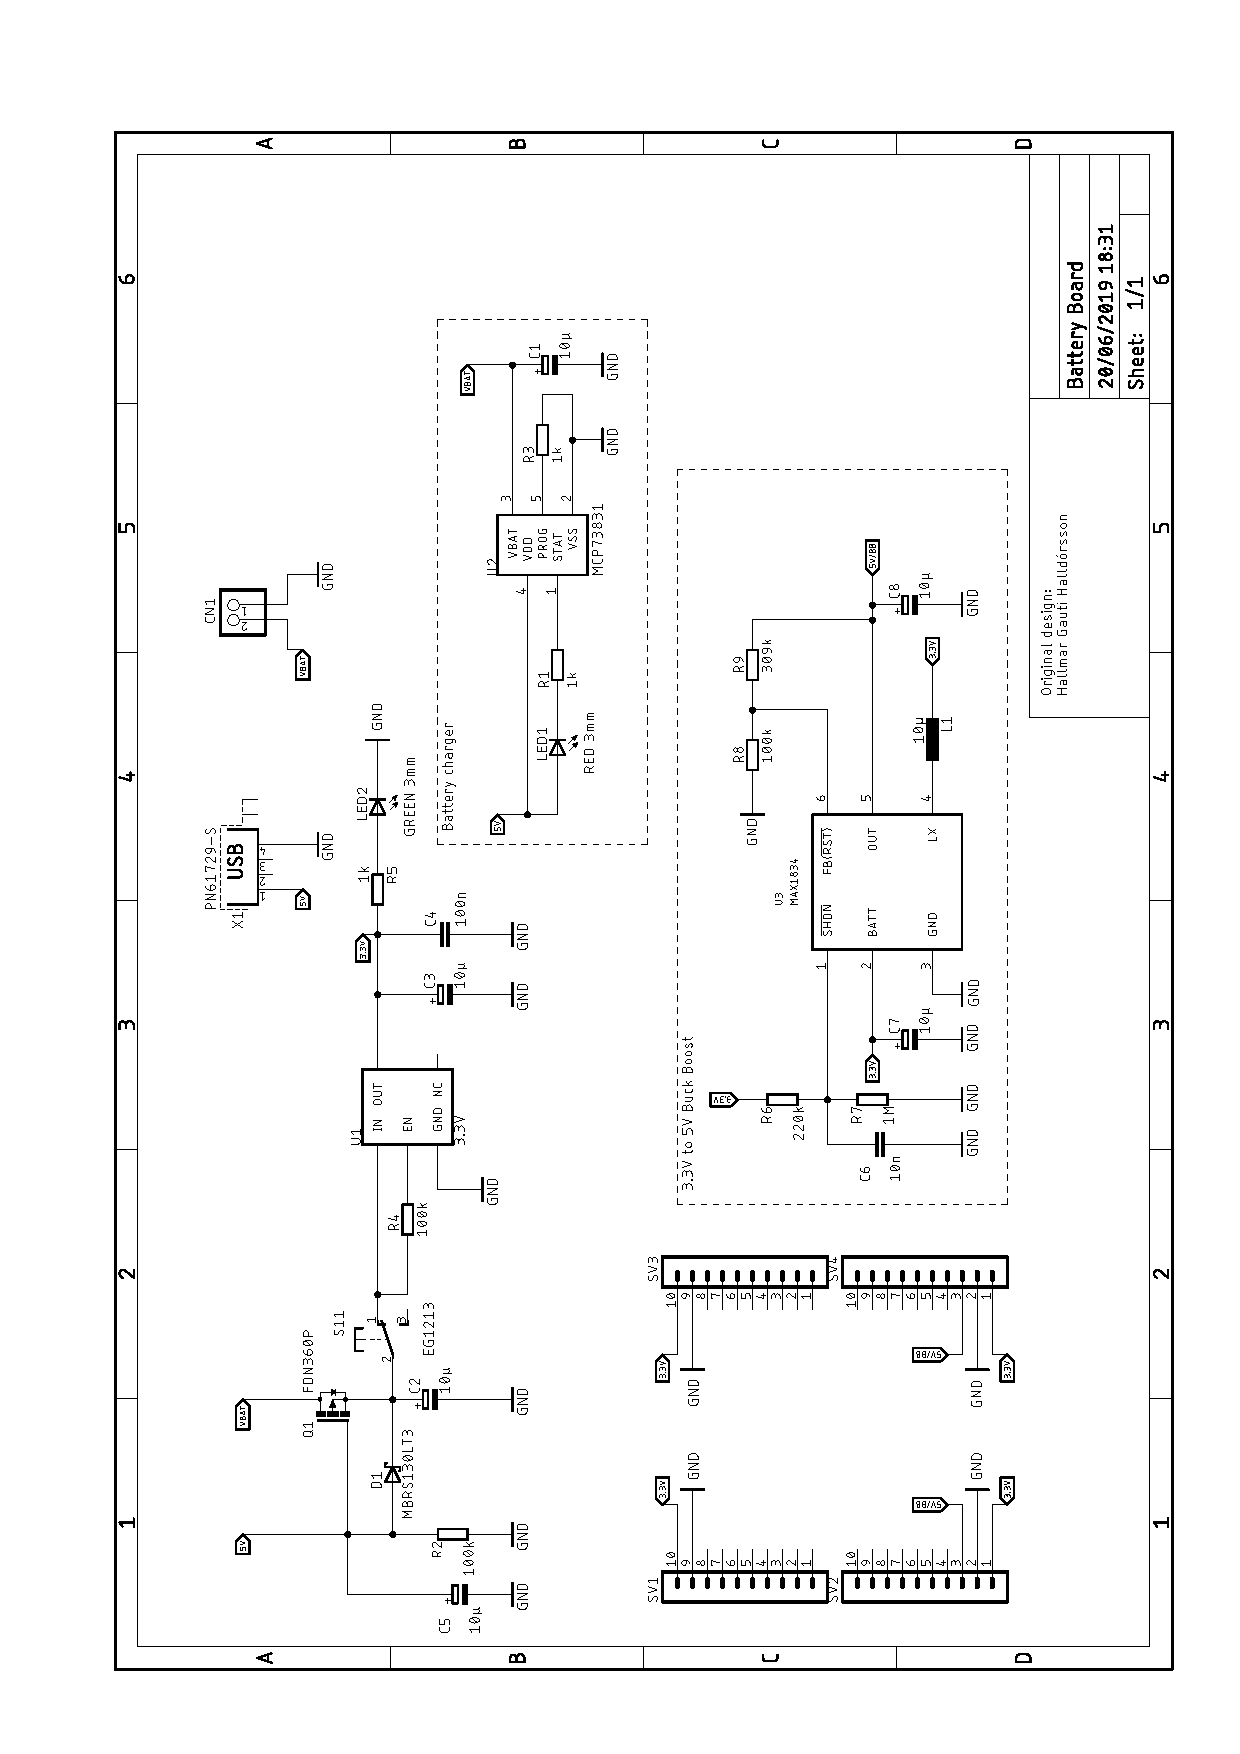
\includegraphics[width=1\linewidth]{battery-b.pdf}
  	\caption{Schematic for PSU board}
 	 \label{fig:schematic2}
\end{figure}
 \subsection{Pictures}
 As can be seen on the picture there is an extra capacitor soldered where the arrow is pointing. This is C8, in this prototype I forgot to put it there which resulted in the 5V to only have an RMS value of around 4.3V. With this C8 the 4.3V jumped up to 5V, as it should be.
  \begin{figure}[H]
  	\centering
  	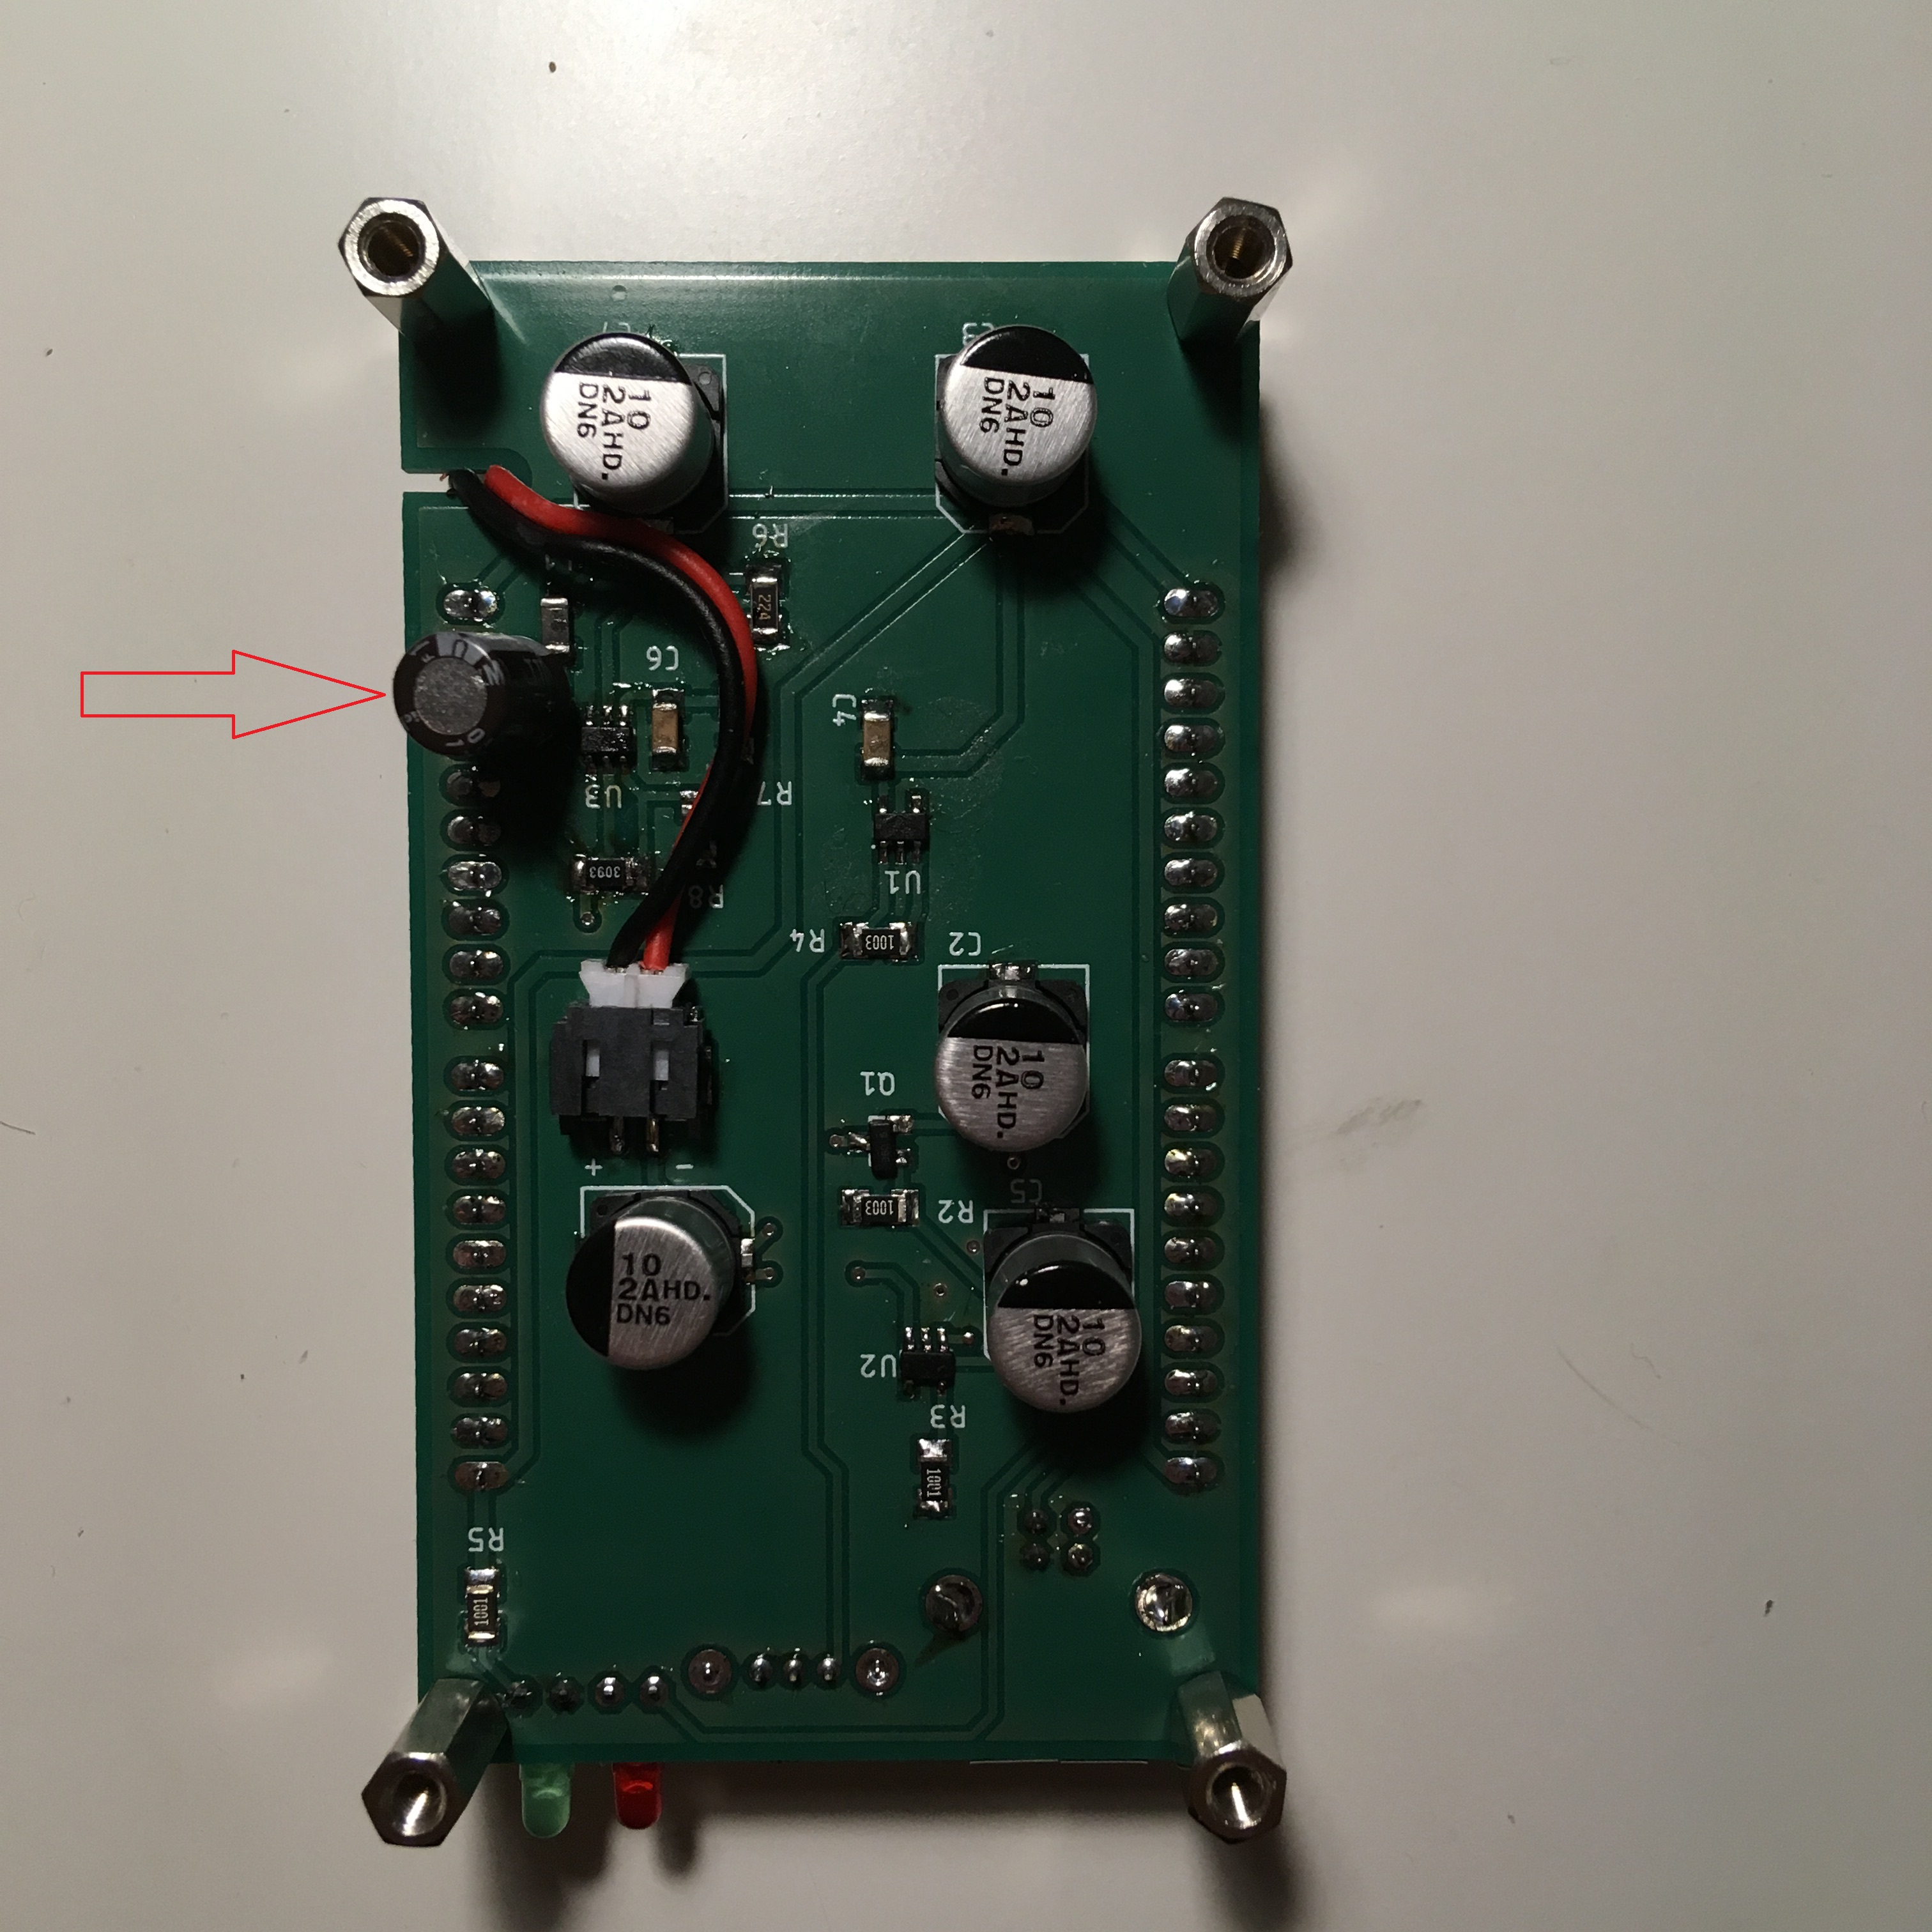
\includegraphics[width=1\linewidth]{IMG_2386.jpg}
  	\caption{Photo of the prototype PCB}
 	 \label{fig: pcb21}
\end{figure}
  \begin{figure}[H]
  	\centering
  	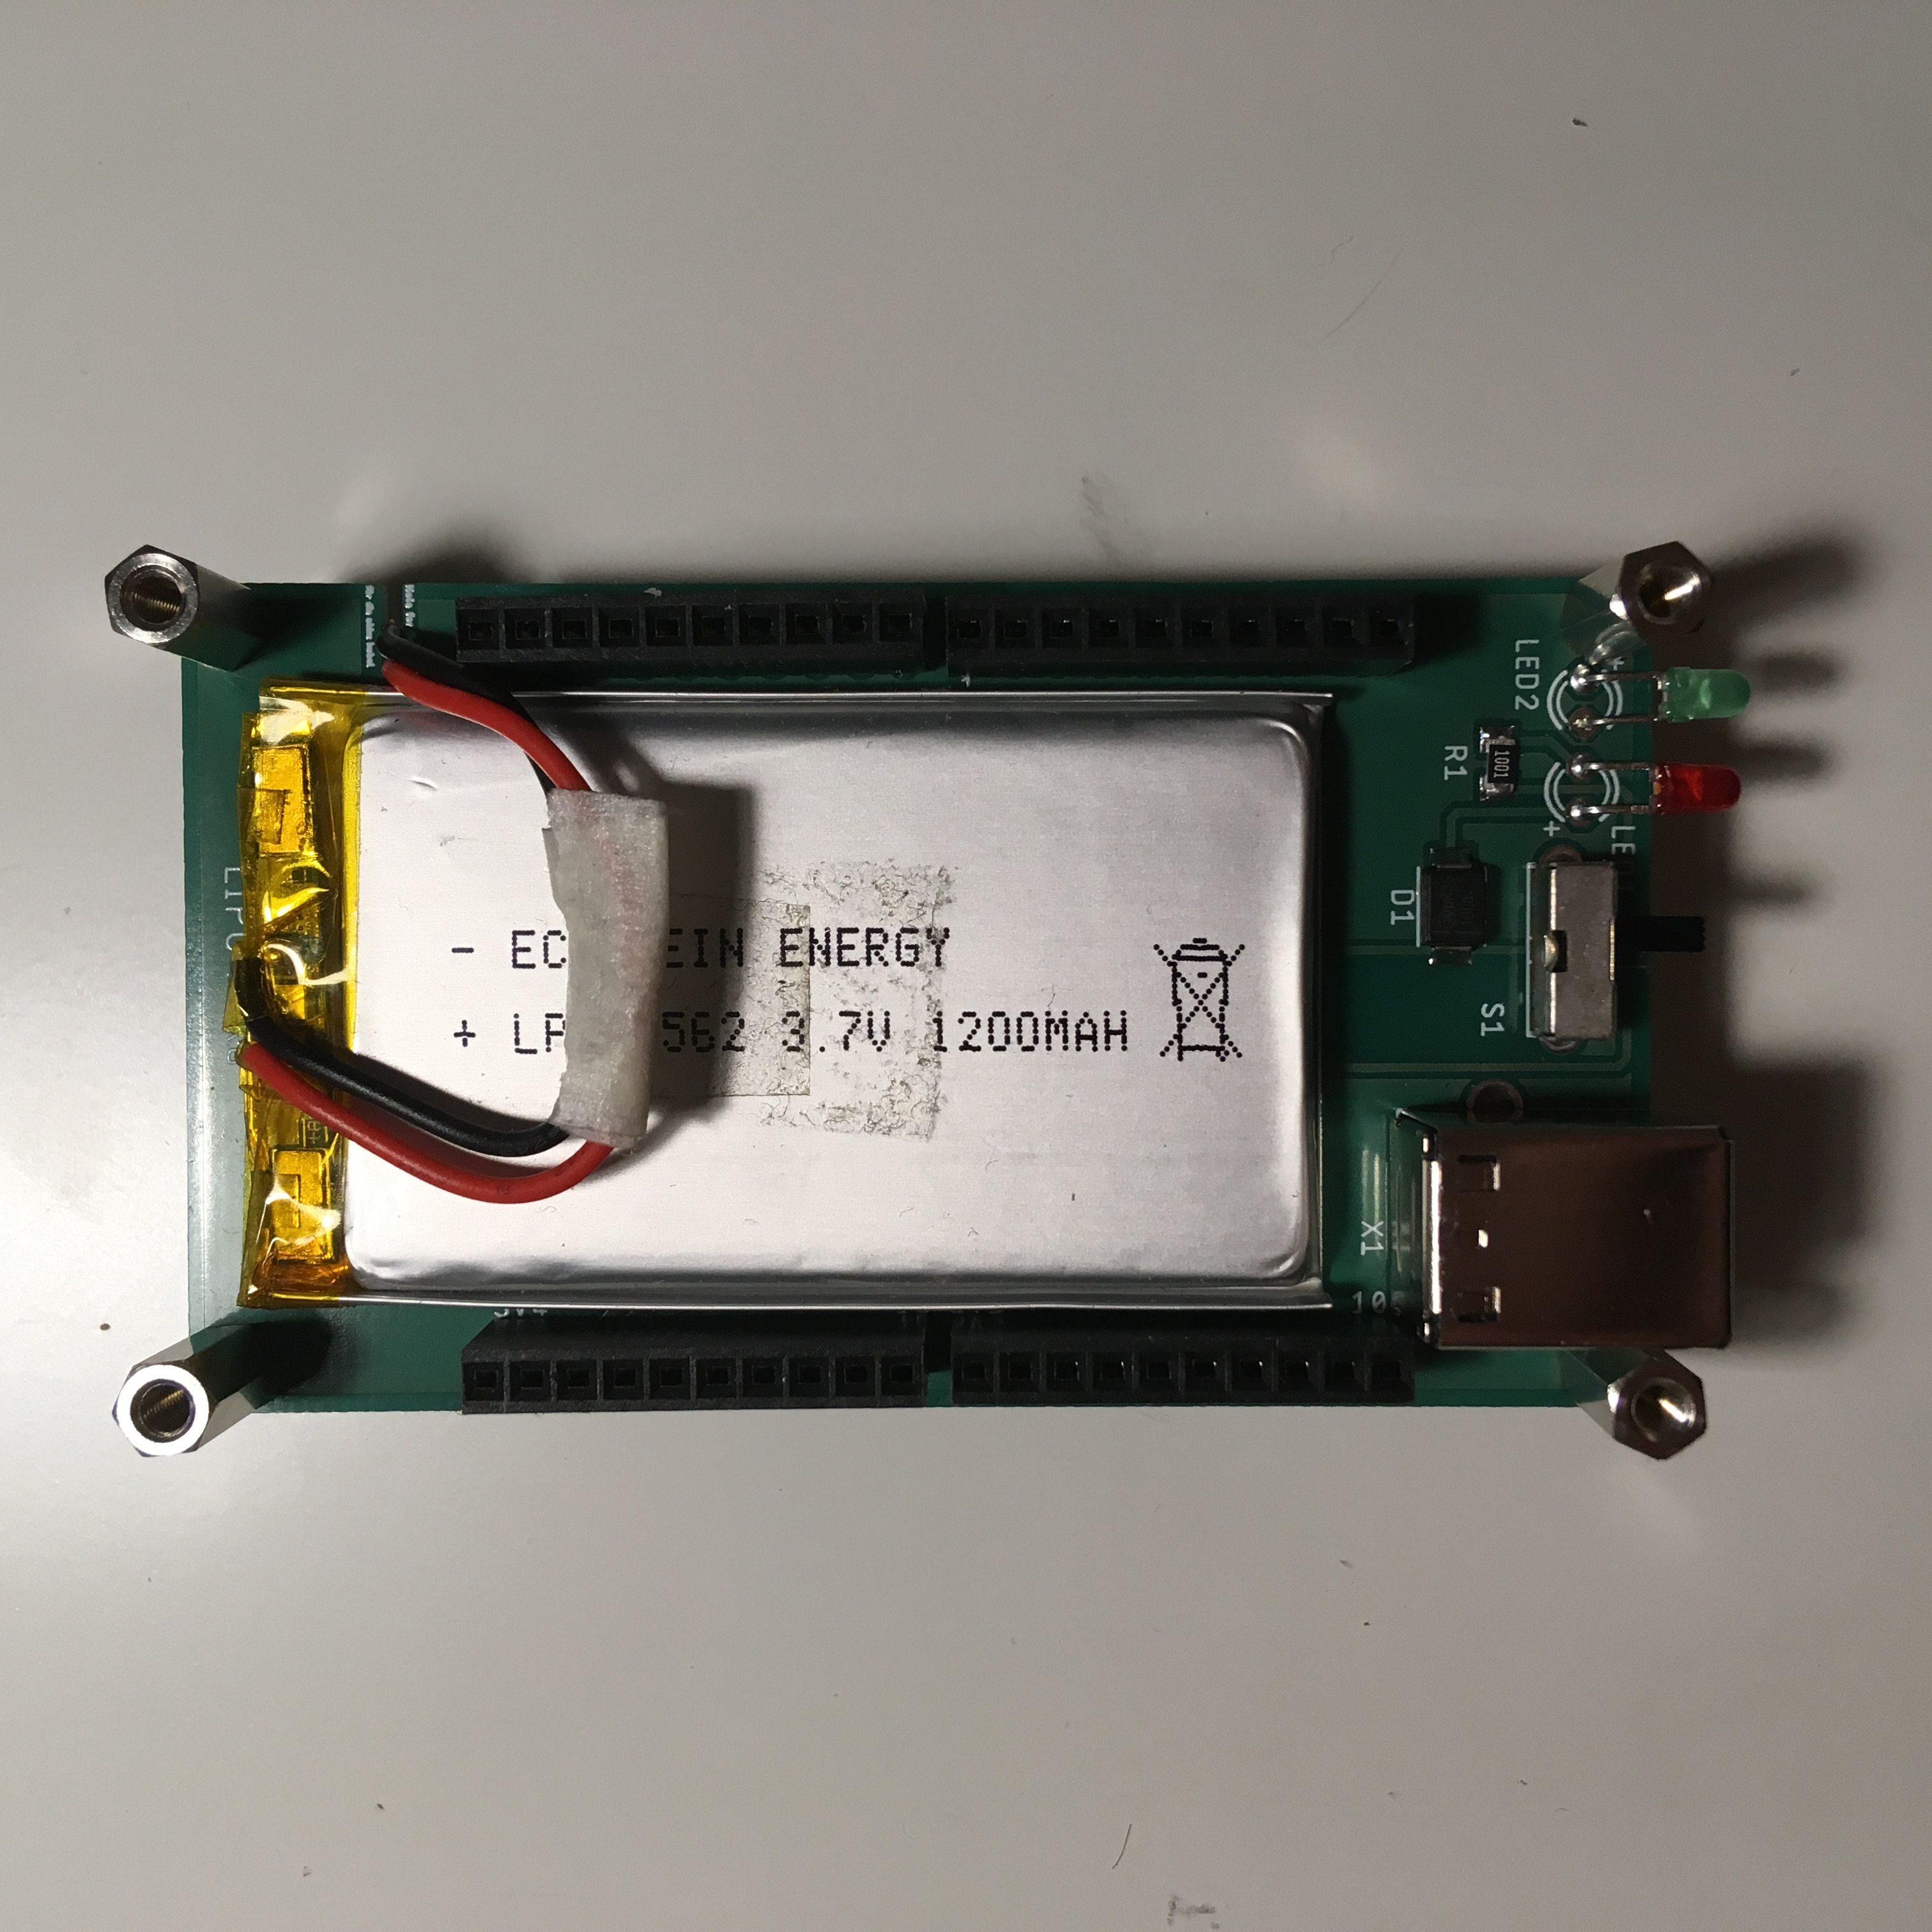
\includegraphics[width=1\linewidth]{IMG_2387.jpg}
  	\caption{Photo of the prototype PCB}
 	 \label{fig: pcb22t}
\end{figure}
 \newpage
 %%%%%%%%%%%%%%%%%%%%%%%%%%%5
 \section{Microcontroller PCB}
 This is the heart of the whole system, here is the Microcontroller that handles everything.
This board also has a  \hyperref[fig: pinout]{prototype header} that can be connected to a breadboard for prototyping all sorts of stuff.
This header has +5V and +3.3V that are limited to 100mA and 150mA respectively.
  \subsection{BOM}
 \begin{center}
    \begin{tabular}{ |m{2em}|m{7em}|m{7em}|m{7em}|}
    \hline
	 \multicolumn{4}{|c|}{\textbf{Microcontroller}} \\
	 \hline
       \textbf{Part} & \textbf{Value} & \textbf{Type} & \textbf{Package} \\ \hline
	R1 & 1k & Resistor & 1206 \\ \hline
	R2 & 1.5k & Resistor & 1206 \\ \hline
	U1 & ESP32-Feather & Microcontroller & -  \\ \hline
	U2 & MIC2009A & Current limiter & SOT-23-6 \\ \hline
	U3 & MIC2009A & Current limiter & SOT-23-6 \\ \hline
	SV1 & 10 pin & Stackable header & Sparkfun: PRT-11376 \\ \hline
	SV2 & 10 pin & Stackable header & Sparkfun: PRT-11376 \\ \hline
	SV3 & 10 pin & Stackable header & Sparkfun: PRT-11376 \\ \hline
	SV4 & 10 pin & Stackable header & Sparkfun: PRT-11376 \\ \hline
	JP3  & 24 pin & 2 row 90° female header & 2.54mm Pitch \\ \hline
    \end{tabular}
     \end{center}
 \newpage
 
      \subsection{Placement}
         \begin{figure}[H]
  	\centering
  	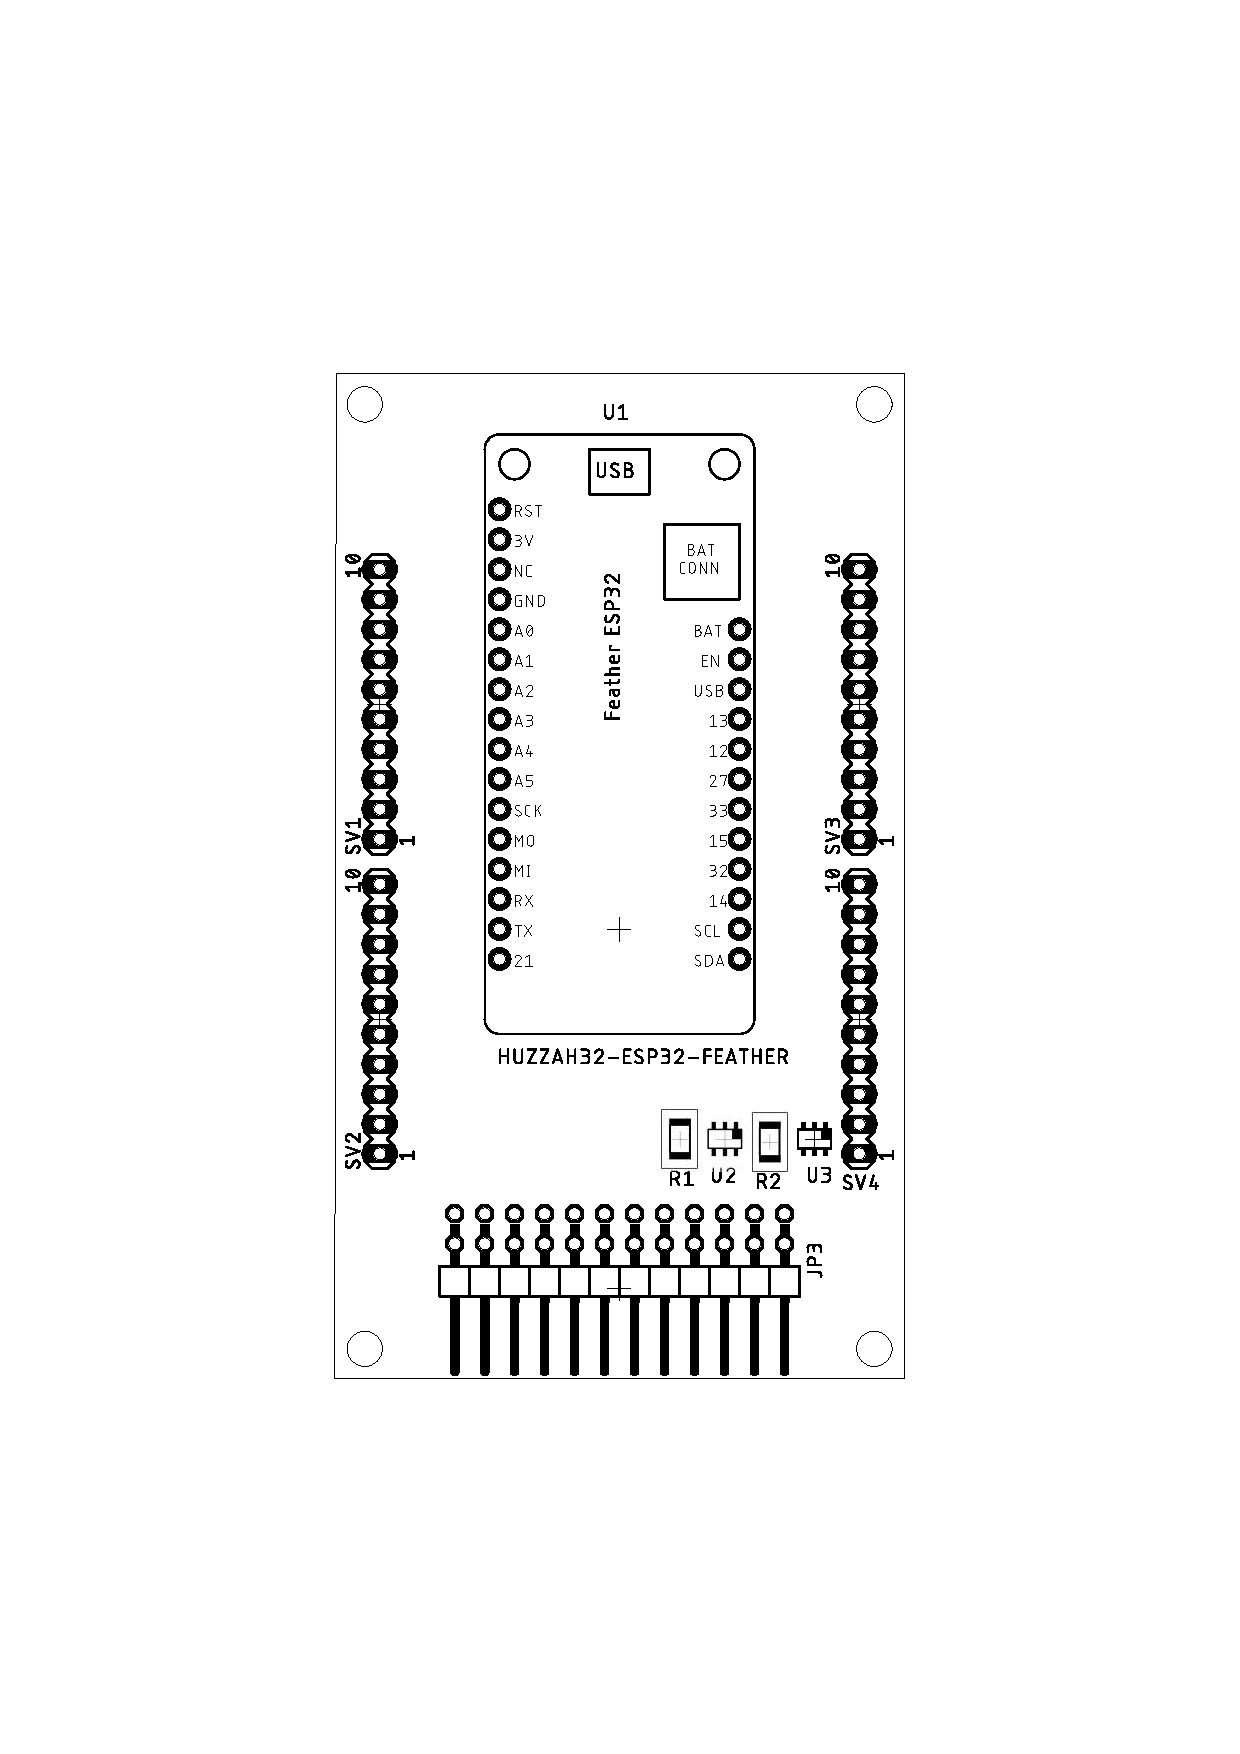
\includegraphics[width=1\linewidth]{mc-placement.pdf}
  	\caption{Placement for Microcontroller board}
 	 \label{fig:place3}
\end{figure}

  \subsection{Schematic}
   \begin{figure}[H]
  	\centering
  	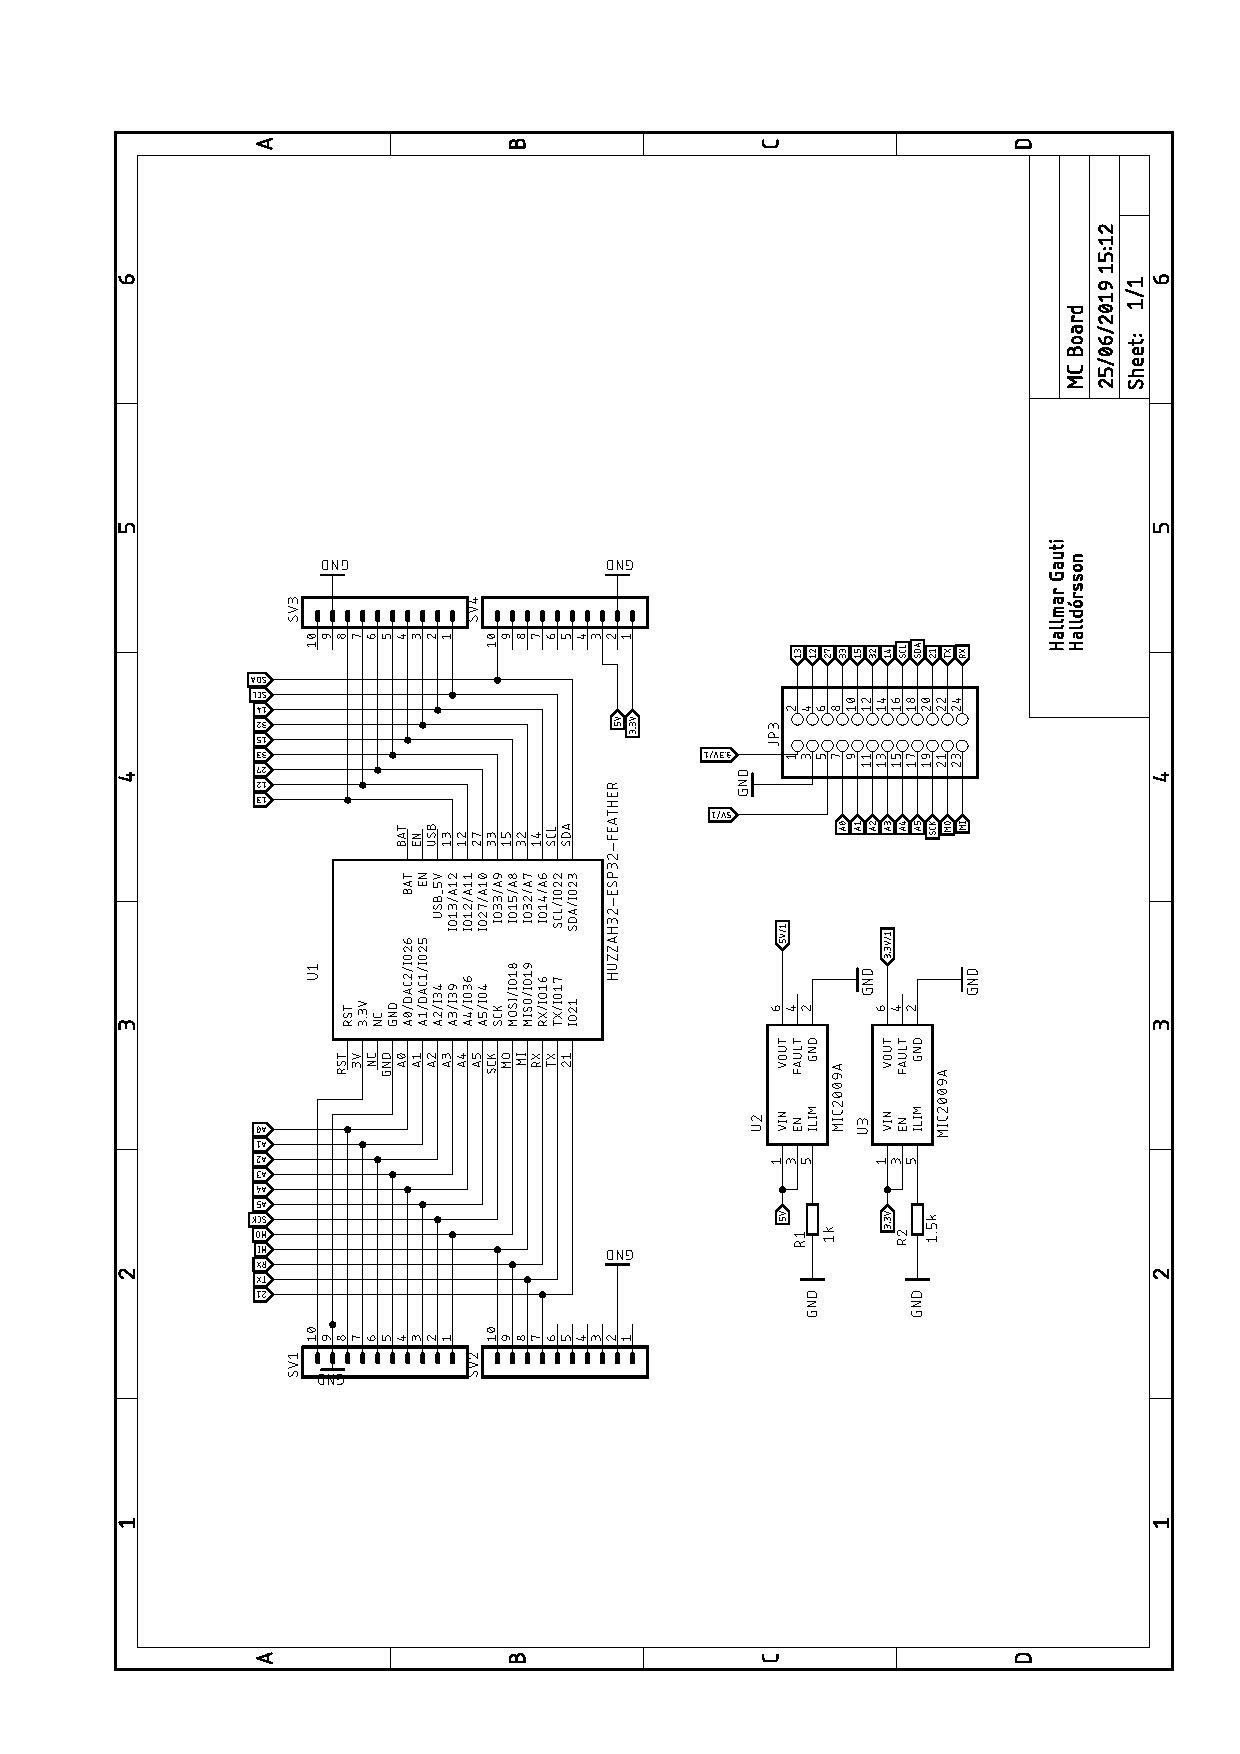
\includegraphics[width=1\linewidth]{microcontroller.pdf}
  	\caption{Schematic for Microcontroller board}
 	 \label{fig:schematic3}
\end{figure}
\newpage

     
 \subsection{Pictures}
 \begin{figure}[H]
  	\centering
  	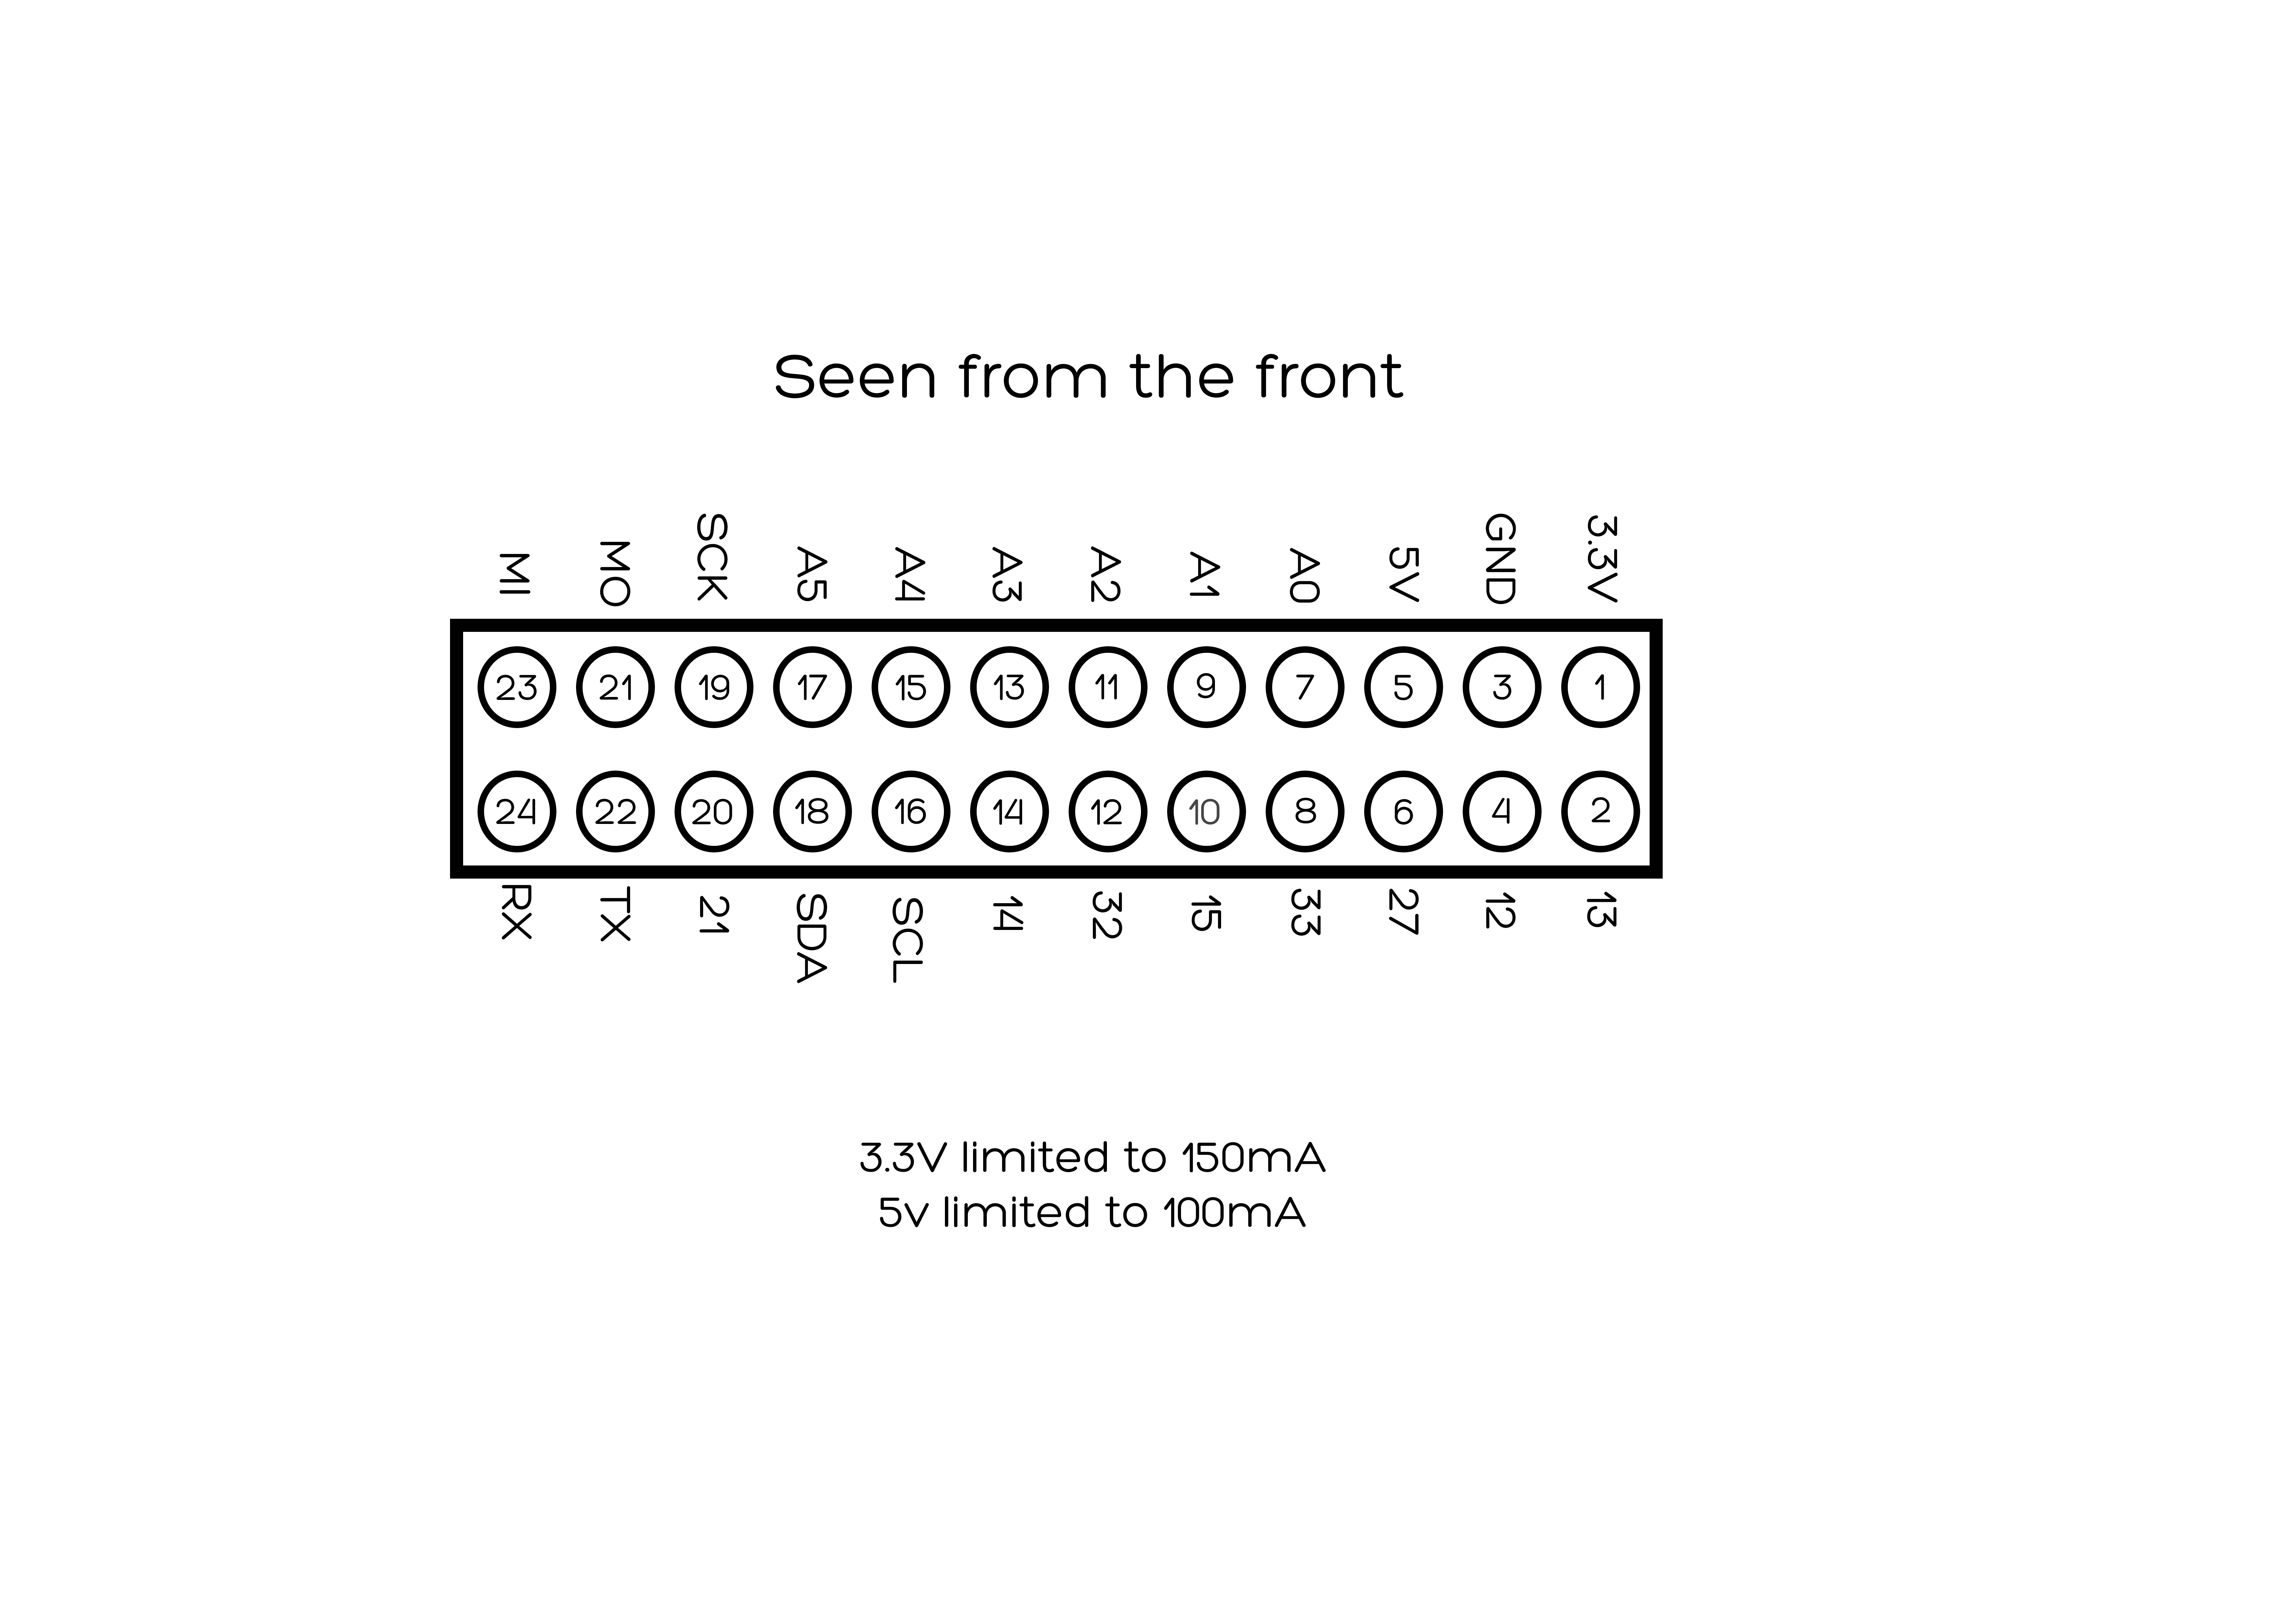
\includegraphics[width=1\linewidth]{Untitled-2.png}
  	\caption{Pinout for Prototyping header}
 	 \label{fig: pinout}
\end{figure}
 \begin{figure}[H]
  	\centering
  	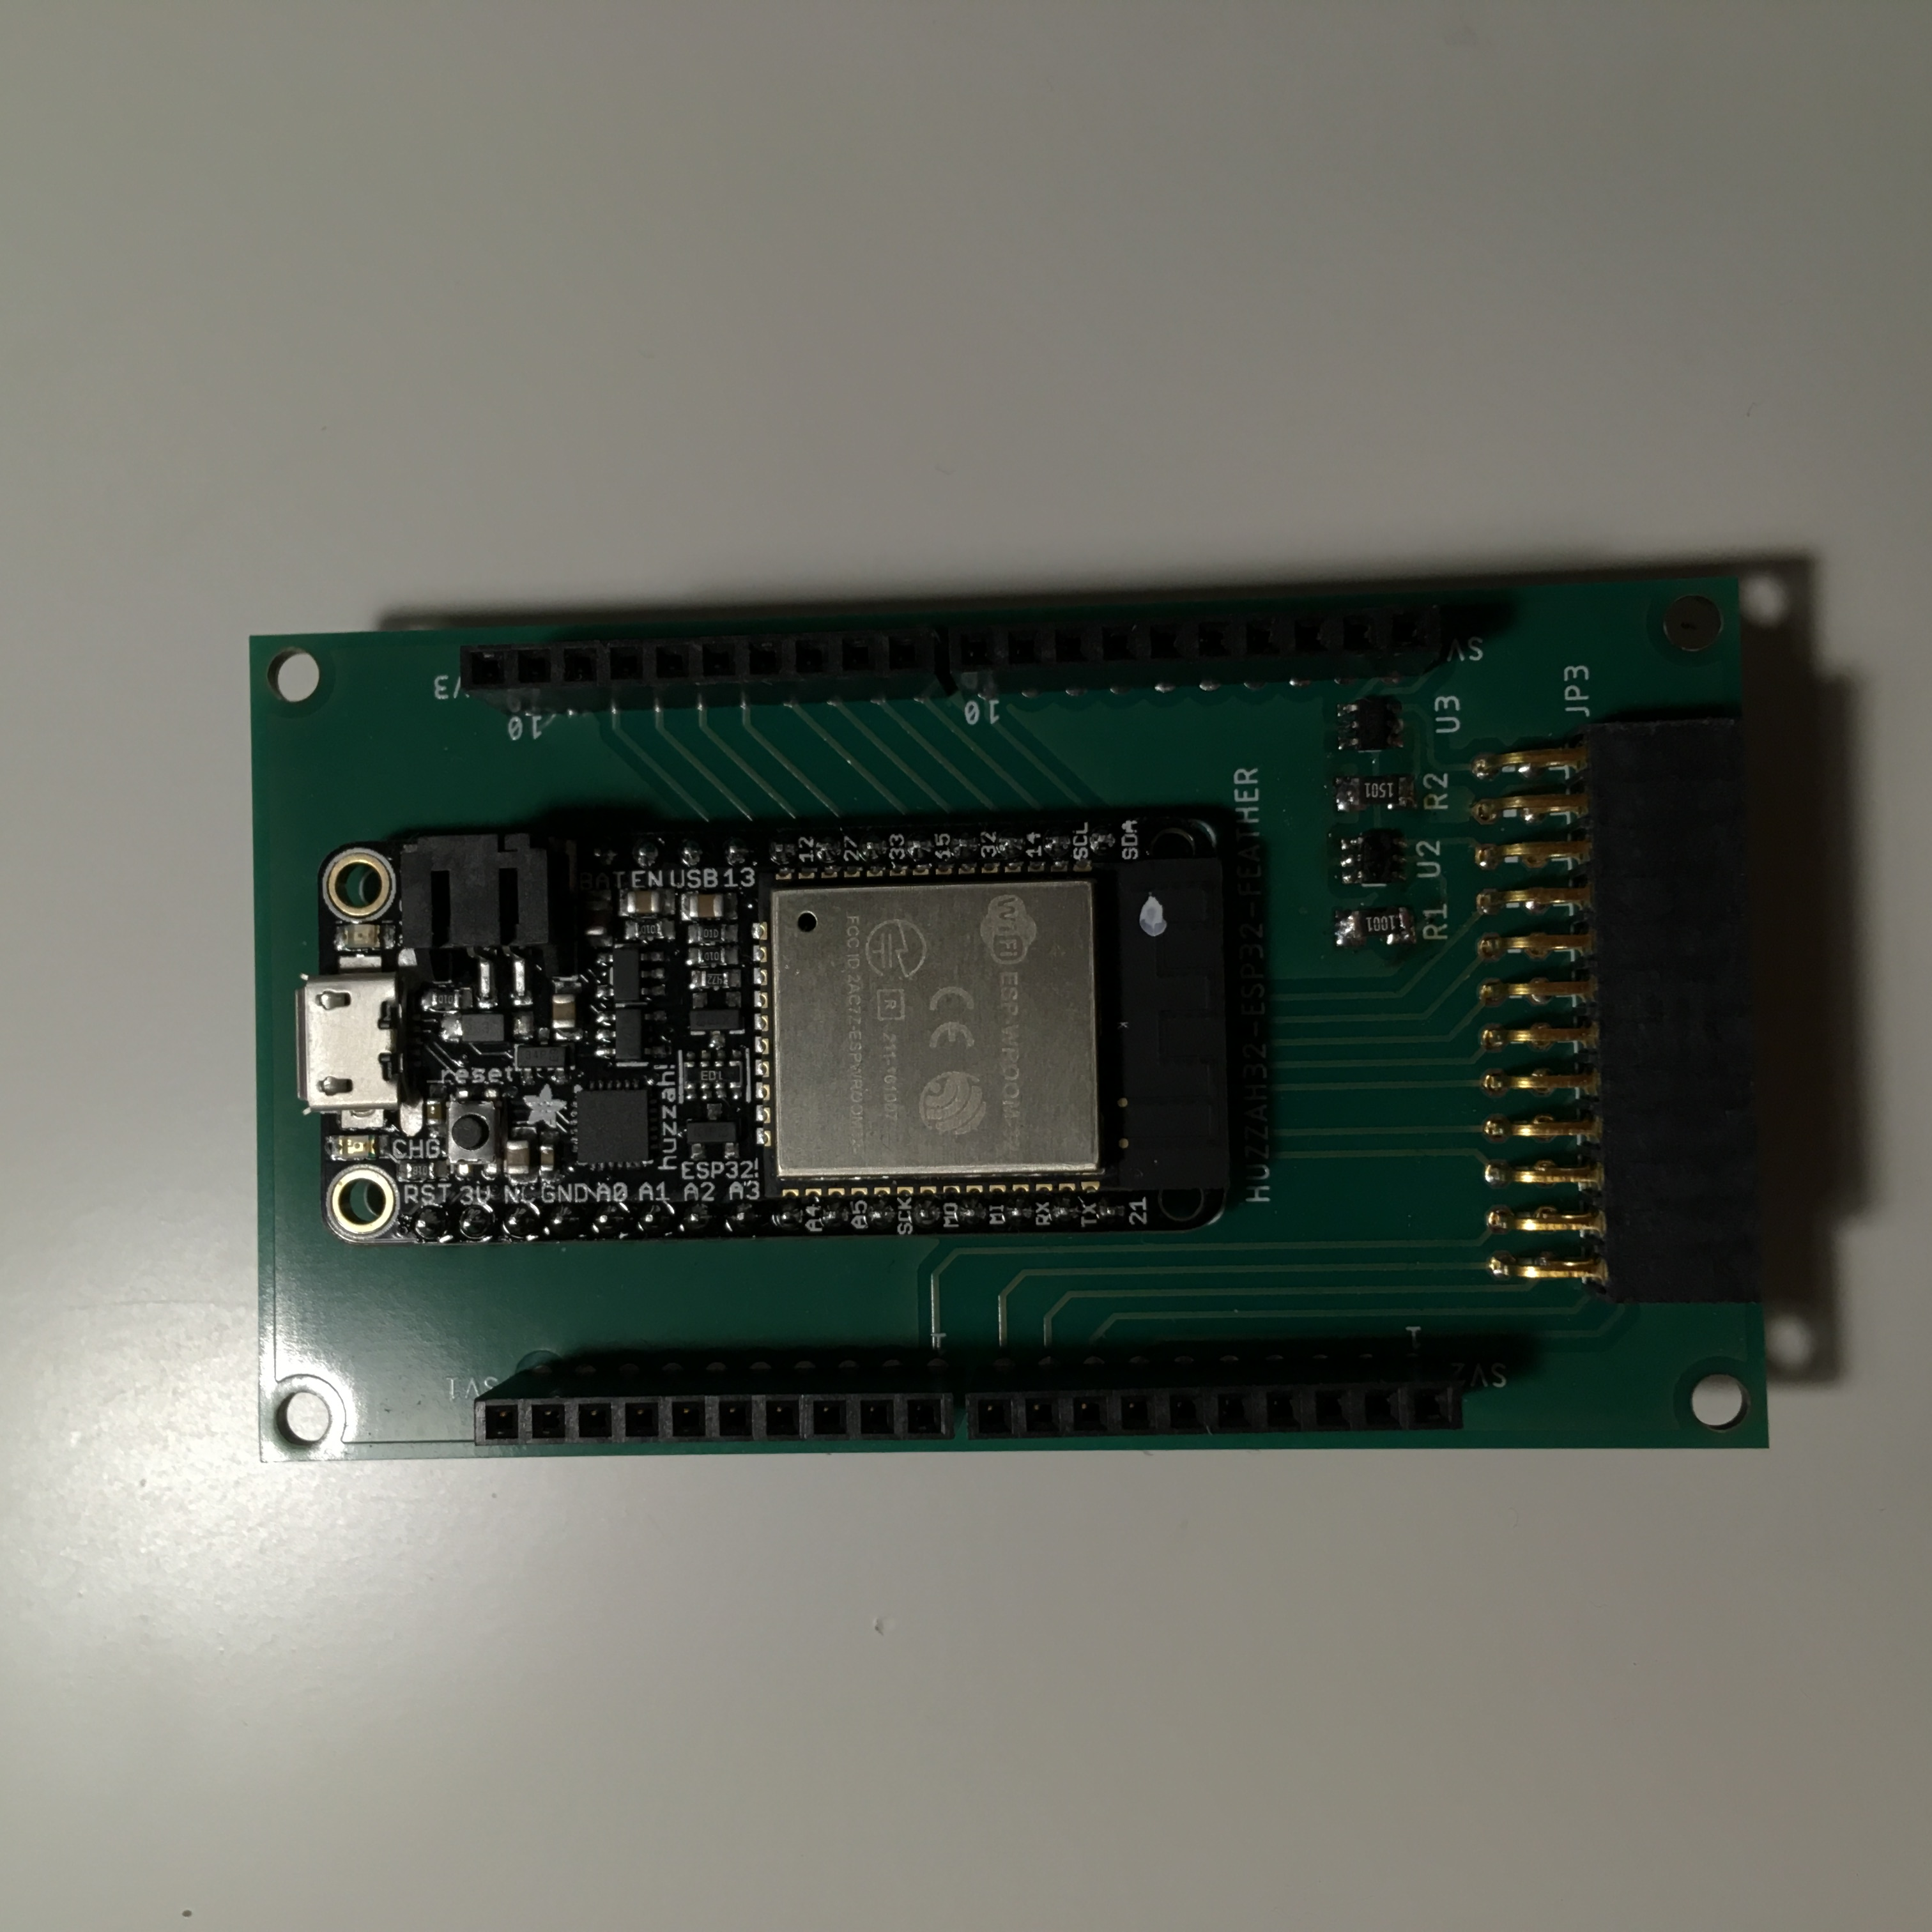
\includegraphics[width=1\linewidth]{IMG_2385.jpg}
  	\caption{PCB prototype}
 	 \label{fig: pcb3}
\end{figure}
\newpage
%%%%%%%%%%%%%%%%%%%%%%%%%%%%%5
\section{HID PCB}
This is the Human Interface Device PCB which has 3 switches, a rotary encoder(with a switch) and an OLED. 
This is all connected to the Microcontroller board. You can see to what pins each component is connected to by looking at the  \hyperref[fig:schematic4]{schematic.}

 \subsection{BOM}
  \begin{center}
    \begin{tabular}{ |m{2em}|m{7em}|m{7em}|m{7em}|}
    \hline
	 \multicolumn{4}{|c|}{\textbf{HID}} \\
	 \hline
       \textbf{Part} & \textbf{Value} & \textbf{Type} & \textbf{Package} \\ \hline
      C1 & 10n & Capacitor & 1206 \\ \hline
      C2 & 10n & Capacitor & 1206 \\ \hline
	R1 & 10k & Resistor & 1206 \\ \hline
	R2 & 10k & Resistor & 1206 \\ \hline
	R3 & 10k & Resistor & 1206 \\ \hline
	R4 & 10k & Resistor & 1206 \\ \hline
	R5 & 10k & Resistor & 1206 \\ \hline
	R6 & 10k & Resistor & 1206 \\ \hline
	R7 & 10k & Resistor & 1206 \\ \hline
	R8 & 10k & Resistor & 1206 \\ \hline
	S1 & TL1105SPF250Q & Tactile Switch & - \\ \hline
	S2 & TL1105SPF250Q & Tactile Switch & -\\ \hline
	S3 & TL1105SPF250Q & Tactile Switch & -\\ \hline
	SW1 & PEC11R-4215F-S0024 & Rotary Ecnoder & - \\ \hline
	U\$1 & Adafruit: 938  & OLED screen & -  \\ \hline
	SV1 & 10 pin & Male header & 2.54mm Pitch \\ \hline
	SV2 & 10 pin & Male header & 2.54mm Pitch \\ \hline
	SV3 & 10 pin & Male header & 2.54mm Pitch \\ \hline
	SV4 & 10 pin & Male header & 2.54mm Pitch \\ \hline
	JP3  & 24 pin & 2 row 90° female header & 2.54mm Pitch \\ \hline

    \end{tabular}
     \end{center}
     
     \subsection{Placement}
         \begin{figure}[H]
  	\centering
  	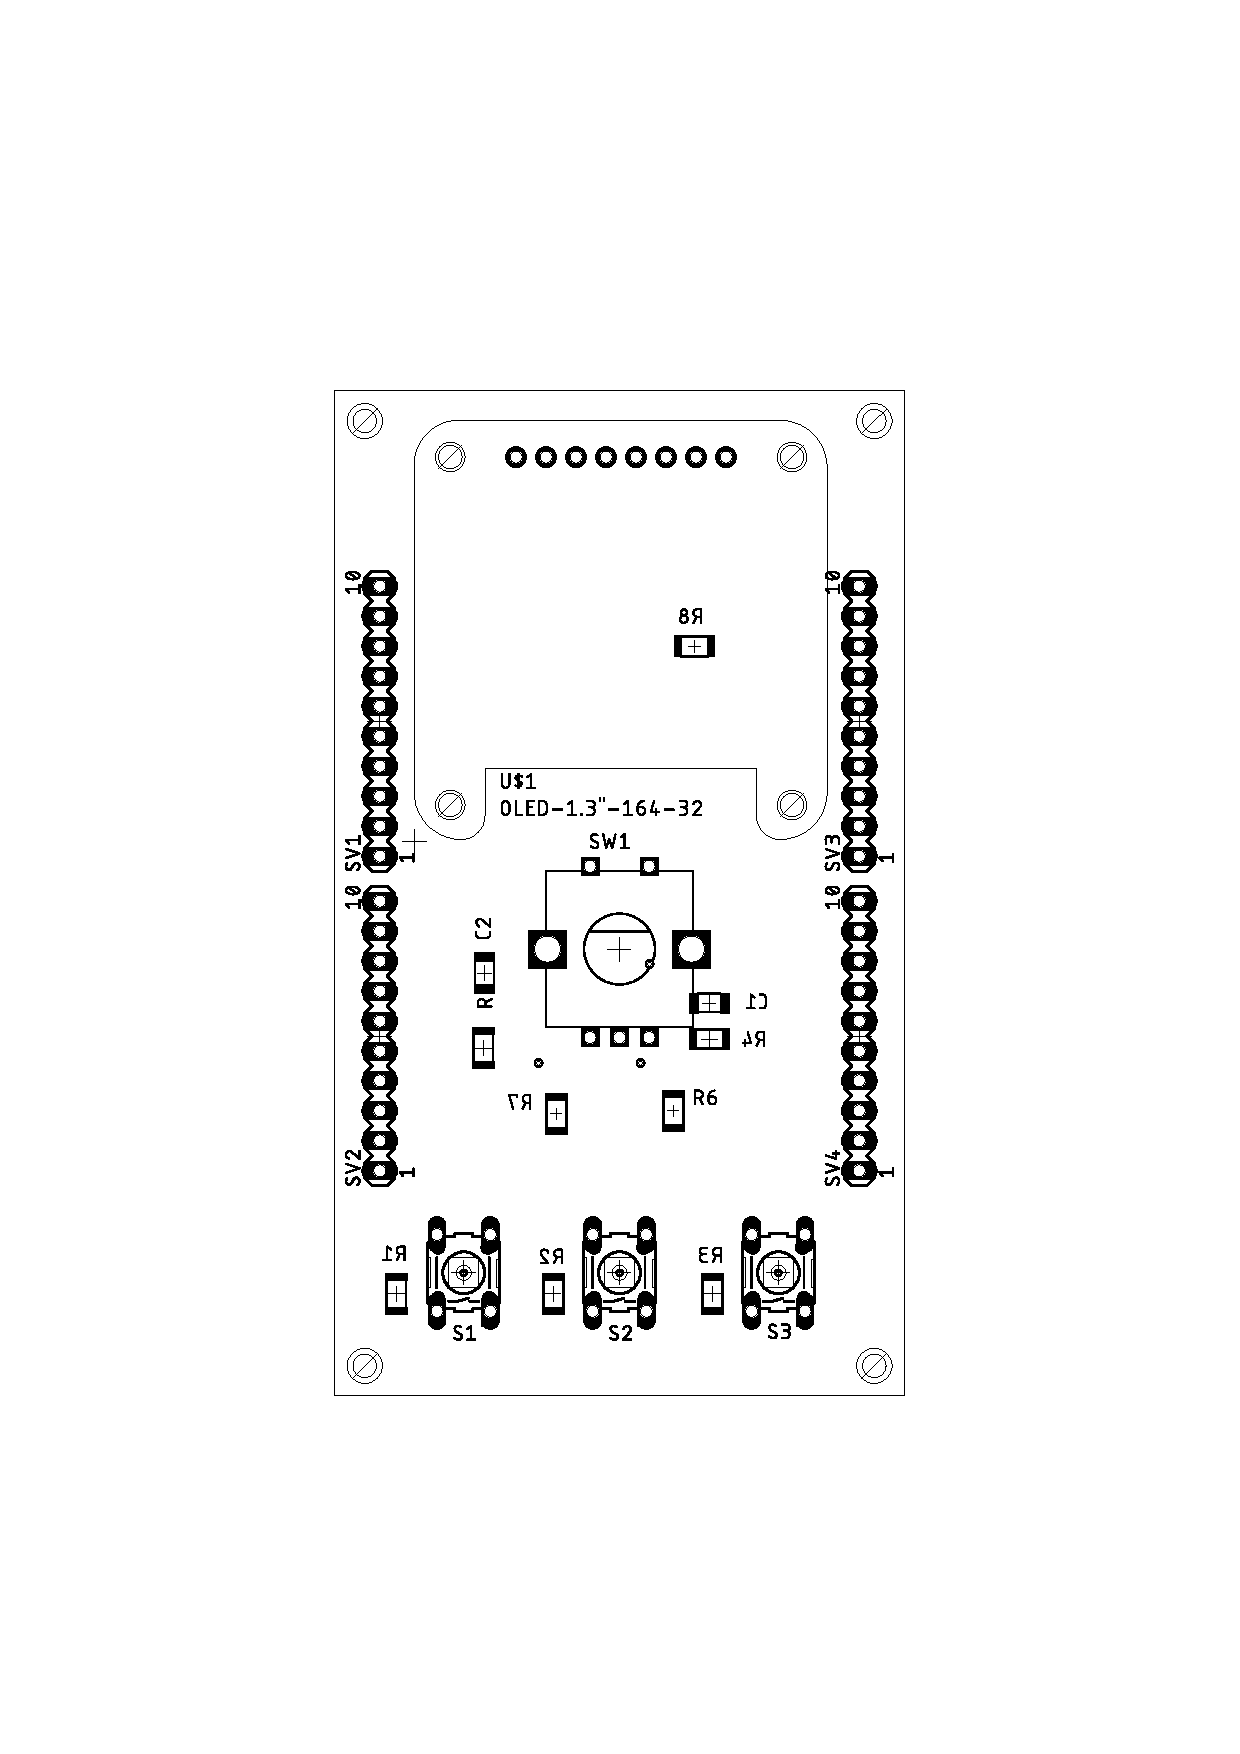
\includegraphics[width=1\linewidth]{OLED-placement.pdf}
  	\caption{Placement for HID board}
 	 \label{fig:place4}
\end{figure}
 \subsection{Schematic}
    \begin{figure}[H]
  	\centering
  	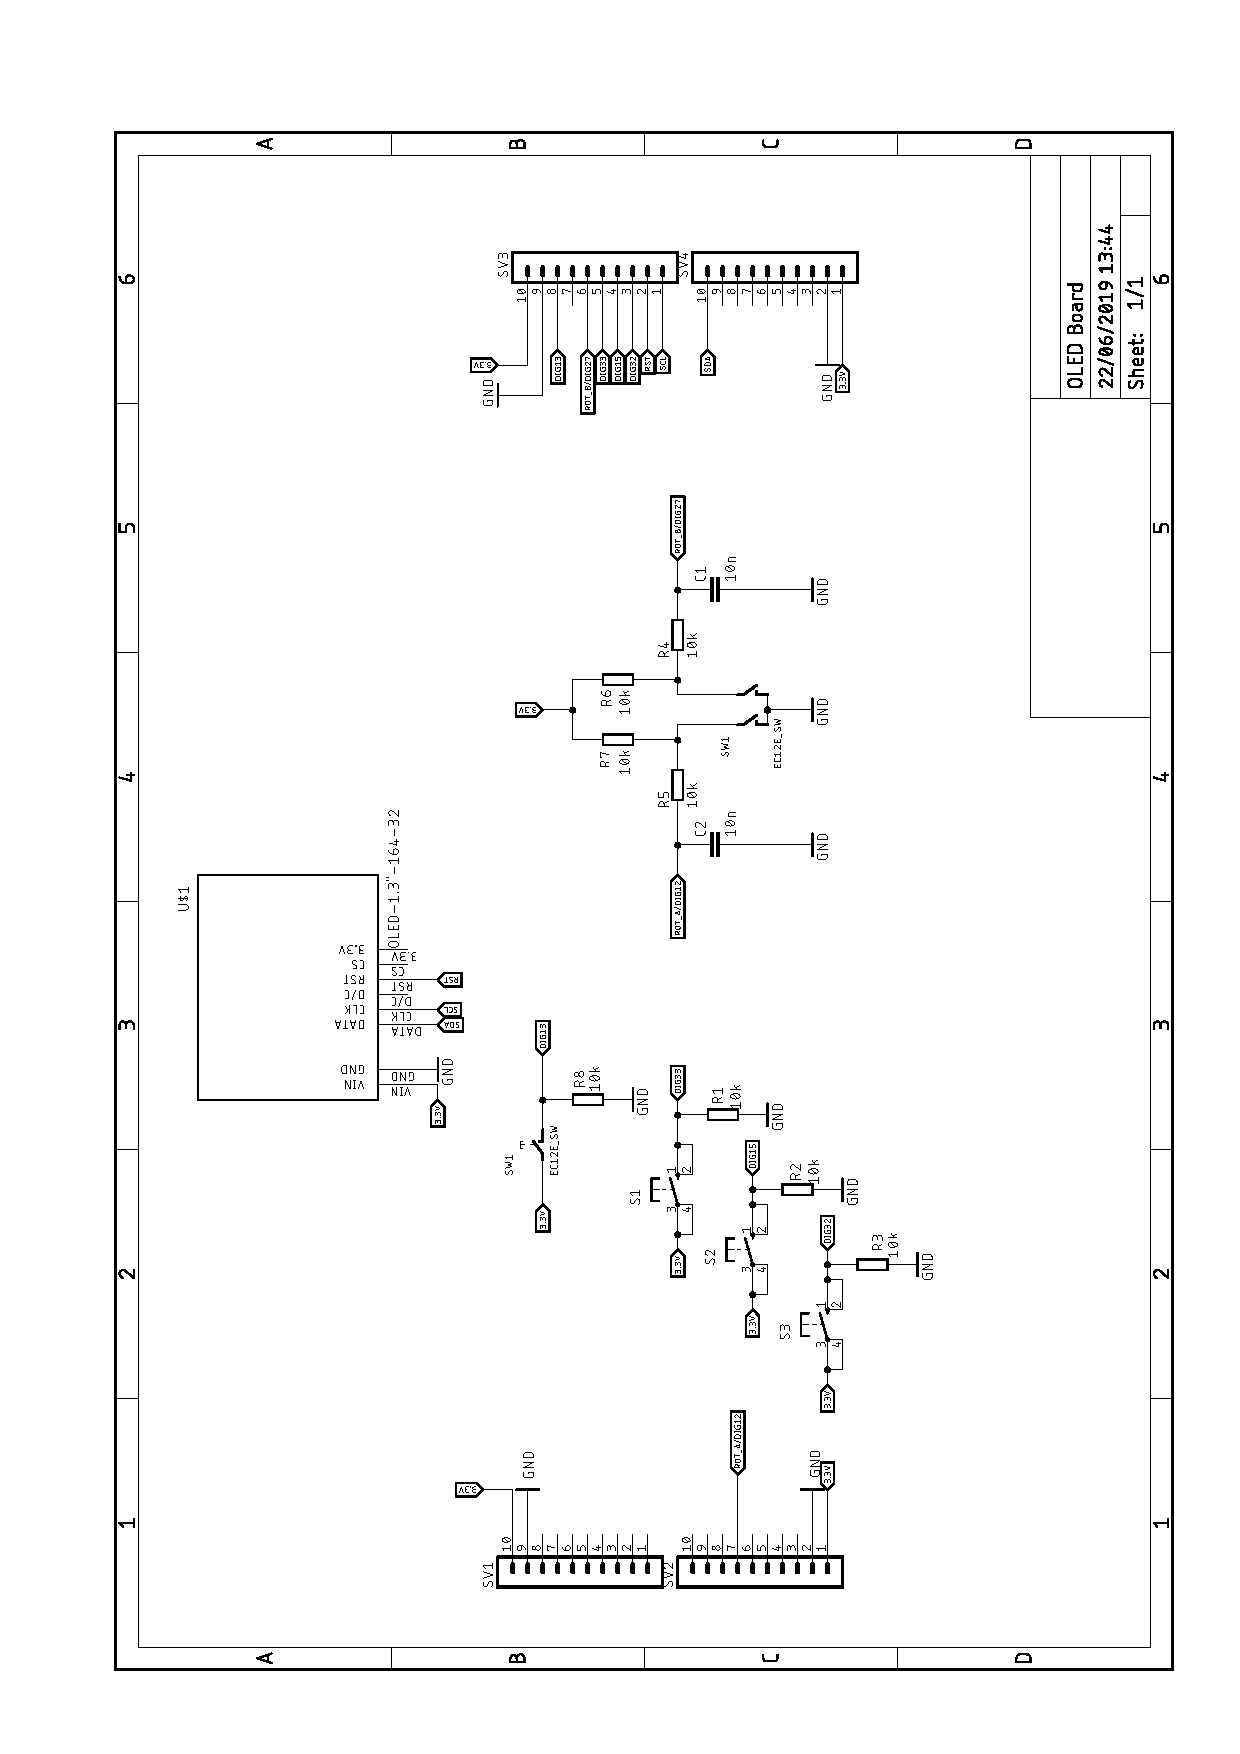
\includegraphics[width=1\linewidth]{OLED-Board.pdf}
  	\caption{Schematic for HID board}
 	 \label{fig:schematic4}
\end{figure}
 \subsection{Pictures}
  \begin{figure}[H]
  	\centering
  	\includegraphics[width=1\linewidth]{IMG_2388.jpg}
  	\caption{Photo of the prototype PCB}
 	 \label{fig:HIDpic}
\end{figure}
  \begin{figure}[H]
  	\centering
  	\includegraphics[width=1\linewidth]{IMG_2389.jpg}
  	\caption{Photo of the prototype PCB}
 	 \label{fig: pcb22t}
\end{figure}

  \begin{figure}[H]
  	\centering
  	\includegraphics[width=1\linewidth]{IMG_2390.jpg}
  	\caption{Photo of the prototype PCB}
 	 \label{fig: pcb22t}
\end{figure}

  \begin{figure}[H]
  	\centering
  	\includegraphics[width=1\linewidth]{IMG_2391.jpg}
  	\caption{Photo of the prototype PCB}
 	 \label{fig: pcb22t}
\end{figure}
\newpage
\section{Peripherals BOM}
Here is a BOM for the peripheral stuff you need, such as screws, standoffs and switch caps. 

  \begin{center}
    \begin{tabular}{ |m{6em}|m{7em}|m{7em}|m{7em}|}
    \hline
	 \multicolumn{4}{|c|}{\textbf{Peripherals}} \\
	 \hline
       \textbf{Amount} & \textbf{Value} & \textbf{Type} & \textbf{Mouser. No} \\ \hline
	3 & 1RBLK & Cap for switches & 1RBLK \\ \hline
	8 & M3 Screw 6mm & Screw & 534-29311 \\ \hline
	12 & 11mm HEX standoff M/F & Standoff & 855-R30-3001102 \\ \hline
	4 & 11mm HEX standoff F/F & Standoff & 855-R30-1001102 \\ \hline
    \end{tabular}
     \end{center}

\section{Links}
Here are some useful (clickable) links for purchasing of the LIPO battery since it cannot be purchased from mouser and some other useful links for the Microcontroller, OLED, some libraries and ect. 
\begin{itemize}
	\item \href{https://www.adafruit.com/product/938}{OLED Display} 
	\item \href{https://learn.adafruit.com/adafruit-huzzah32-esp32-feather?view=all}{ESP32 Feather platform Information}
	\item \href{https://learn.adafruit.com/adafruit-huzzah32-esp32-feather/using-with-arduino-ide}{Using ESP32 Feather with Arduino IDE}
	\item \href{https://randomnerdtutorials.com/esp32-access-point-ap-web-server/}{Access Point Tutorial for ESP32}
	\item \href{https://randomnerdtutorials.com/esp32-web-server-arduino-ide/}{Web server Tutorial for ESP32}
	\item \href{https://github.com/ThingPulse/esp8266-oled-ssd1306}{Library for Adafruit OLED}
	\item \href{https://github.com/adafruit/Adafruit-GFX-Library}{Library for Adafruit OLED(GFX)}
	\item \href{https://www.adafruit.com/product/258}{LIPO battery on Adafruit} 
	\item 	\href{https://eckstein-shop.de/LiPo-Akku-Lithium-Ion-Polymer-Batterie-37V-1200mAh-JST-PH-Connector?curr=EUR&gclid=Cj0KCQiAxNnfBRDwARIsAJlH29BLePjR8XtucLdkk6RyHy8WfTtGj7G8zkp6dZxTWrhhOybtX9XS7-0aAmj1EALw_wcB}{Purchase LIPO Battery in Europe}
	\item \href{https://www.mouser.com/ProjectManager/ProjectDetail.aspx?AccessID=9a8a02e45e}{Mouser Cart}
\end{itemize}

\end{document}